
\documentclass[spanish,openright]{book}

\usepackage[utf8]{inputenc}
\usepackage[english]{babel}
\usepackage{graphicx}
\usepackage[nottoc]{tocbibind} % para que muestre el apartado de referencias en el índice
\usepackage{lipsum} % Para meter texto random
%%%%%%%%%%%%%%%%%%%%%%%%%%%%%%%
% CONFIGURACIÓN CÓDIGO PYTHON %
%%%%%%%%%%%%%%%%%%%%%%%%%%%%%%%

% Estilo del codigo escrito en el documento

\definecolor{maroon}{cmyk}{0, 0.87, 0.68, 0.32}
\definecolor{halfgray}{gray}{0.55}
\definecolor{ipython_frame}{RGB}{207, 207, 207}
\definecolor{ipython_bg}{RGB}{247, 247, 247}
\definecolor{ipython_red}{RGB}{186, 33, 33}
\definecolor{ipython_green}{RGB}{0, 128, 0}
\definecolor{ipython_cyan}{RGB}{64, 128, 128}
\definecolor{ipython_purple}{RGB}{170, 34, 255}

\usepackage{listings}
\lstset{
    breaklines=true,
    xleftmargin=.29in,
    xrightmargin=.29in,
    extendedchars=true,
    literate=
    {á}{{\'a}}1 {é}{{\'e}}1 {í}{{\'i}}1 {ó}{{\'o}}1 {ú}{{\'u}}1
    {Á}{{\'A}}1 {É}{{\'E}}1 {Í}{{\'I}}1 {Ó}{{\'O}}1 {Ú}{{\'U}}1
    {à}{{\`a}}1 {è}{{\`e}}1 {ì}{{\`i}}1 {ò}{{\`o}}1 {ù}{{\`u}}1
    {À}{{\`A}}1 {È}{{\'E}}1 {Ì}{{\`I}}1 {Ò}{{\`O}}1 {Ù}{{\`U}}1
    {ä}{{\"a}}1 {ë}{{\"e}}1 {ï}{{\"i}}1 {ö}{{\"o}}1 {ü}{{\"u}}1
    {Ä}{{\"A}}1 {Ë}{{\"E}}1 {Ï}{{\"I}}1 {Ö}{{\"O}}1 {Ü}{{\"U}}1
    {â}{{\^a}}1 {ê}{{\^e}}1 {î}{{\^i}}1 {ô}{{\^o}}1 {û}{{\^u}}1
    {Â}{{\^A}}1 {Ê}{{\^E}}1 {Î}{{\^I}}1 {Ô}{{\^O}}1 {Û}{{\^U}}1
    {œ}{{\oe}}1 {Œ}{{\OE}}1 {æ}{{\ae}}1 {Æ}{{\AE}}1 {ß}{{\ss}}1
    {ç}{{\c c}}1 {Ç}{{\c C}}1 {ø}{{\o}}1 {å}{{\r a}}1 {Å}{{\r A}}1
    {€}{{\EUR}}1 {£}{{\pounds}}1
}

%%
%% Python definition (c) 1998 Michael Weber
%% Additional definitions (2013) Alexis Dimitriadis
%% modified by me (should not have empty lines)
%%
\lstdefinelanguage{iPython}{
    morekeywords={access,and,break,class,continue,def,del,elif,else,except,exec,finally,for,from,global,if,import,in,is,lambda,not,or,pass,print,raise,return,try,while},%
    %
    % Built-ins
    morekeywords=[2]{abs,all,any,basestring,bin,bool,bytearray,callable,chr,classmethod,cmp,compile,complex,delattr,dict,dir,divmod,enumerate,eval,execfile,file,filter,float,format,frozenset,getattr,globals,hasattr,hash,help,hex,id,input,int,isinstance,issubclass,iter,len,list,locals,long,map,max,memoryview,min,next,object,oct,open,ord,pow,property,range,raw_input,reduce,reload,repr,reversed,round,set,setattr,slice,sorted,staticmethod,str,sum,super,tuple,type,unichr,unicode,vars,xrange,zip,apply,buffer,coerce,intern},%
    %
    sensitive=true,%
    morecomment=[l]\#,%
    morestring=[b]',%
    morestring=[b]",%
    %
    morestring=[s]{'''}{'''},% used for documentation text (mulitiline strings)
    morestring=[s]{"""}{"""},% added by Philipp Matthias Hahn
    %
    morestring=[s]{r'}{'},% `raw' strings
    morestring=[s]{r"}{"},%
    morestring=[s]{r'''}{'''},%
    morestring=[s]{r"""}{"""},%
    morestring=[s]{u'}{'},% unicode strings
    morestring=[s]{u"}{"},%
    morestring=[s]{u'''}{'''},%
    morestring=[s]{u"""}{"""},%
    %
    % {replace}{replacement}{lenght of replace}
    % *{-}{-}{1} will not replace in comments and so on
    literate=
    {á}{{\'a}}1 {é}{{\'e}}1 {í}{{\'i}}1 {ó}{{\'o}}1 {ú}{{\'u}}1
    {Á}{{\'A}}1 {É}{{\'E}}1 {Í}{{\'I}}1 {Ó}{{\'O}}1 {Ú}{{\'U}}1
    {à}{{\`a}}1 {è}{{\`e}}1 {ì}{{\`i}}1 {ò}{{\`o}}1 {ù}{{\`u}}1
    {À}{{\`A}}1 {È}{{\'E}}1 {Ì}{{\`I}}1 {Ò}{{\`O}}1 {Ù}{{\`U}}1
    {ä}{{\"a}}1 {ë}{{\"e}}1 {ï}{{\"i}}1 {ö}{{\"o}}1 {ü}{{\"u}}1
    {Ä}{{\"A}}1 {Ë}{{\"E}}1 {Ï}{{\"I}}1 {Ö}{{\"O}}1 {Ü}{{\"U}}1
    {â}{{\^a}}1 {ê}{{\^e}}1 {î}{{\^i}}1 {ô}{{\^o}}1 {û}{{\^u}}1
    {Â}{{\^A}}1 {Ê}{{\^E}}1 {Î}{{\^I}}1 {Ô}{{\^O}}1 {Û}{{\^U}}1
    {œ}{{\oe}}1 {Œ}{{\OE}}1 {æ}{{\ae}}1 {Æ}{{\AE}}1 {ß}{{\ss}}1
    {ç}{{\c c}}1 {Ç}{{\c C}}1 {ø}{{\o}}1 {å}{{\r a}}1 {Å}{{\r A}}1
    {€}{{\EUR}}1 {£}{{\pounds}}1,
    %
    literate=
    *{+}{{{\color{ipython_purple}+}}}1
    {-}{{{\color{ipython_purple}-}}}1
    {*}{{{\color{ipython_purple}$^\ast$}}}1
    {/}{{{\color{ipython_purple}/}}}1
    {^}{{{\color{ipython_purple}\^{}}}}1
    {?}{{{\color{ipython_purple}?}}}1
    {!}{{{\color{ipython_purple}!}}}1
    {\%}{{{\color{ipython_purple}\%}}}1
    {<}{{{\color{ipython_purple}<}}}1
    {>}{{{\color{ipython_purple}>}}}1
    {|}{{{\color{ipython_purple}|}}}1
    {\&}{{{\color{ipython_purple}\&}}}1
    {~}{{{\color{ipython_purple}~}}}1
    %
    {==}{{{\color{ipython_purple}==}}}2
    {<=}{{{\color{ipython_purple}<=}}}2
    {>=}{{{\color{ipython_purple}>=}}}2
    %
    {+=}{{{+=}}}2
    {-=}{{{-=}}}2
    {*=}{{{$^\ast$=}}}2
    {/=}{{{/=}}}2,
    %
%   identifierstyle=\color{red}\ttfamily,
    commentstyle=\color{ipython_cyan}\ttfamily,
    stringstyle=\color{ipython_red}\ttfamily,
    keepspaces=true,
    showspaces=false,
    showstringspaces=false,
    %
    rulecolor=\color{ipython_frame},
    frame=single,
    frameround={t}{t}{t}{t},
    framexleftmargin=6mm,
    numbers=left,
    numberstyle=\tiny\color{halfgray},
    %
    %
    backgroundcolor=\color{ipython_bg},
    %   extendedchars=true,
    basicstyle=\scriptsize\ttfamily,
    keywordstyle=\color{ipython_green}\ttfamily,
    escapechar=\¢,escapebegin=\color{ipython_green},
}

\makeglossaries % Genera la base de datos de acrónimos
\newacronym{aboda}{ABODA}{Abandoned Objects Dataset}
\newacronym{doa}{DOA}{Detección de Objetos Abandonados}
\newacronym{ap}{AP}{Average precision}
\newacronym{asff}{ASFF}{Adaptively Spatial Feature Fusion}
\newacronym{auc}{AUC}{Area Under the ROC Curve}
\newacronym{avss}{AVSSAB2007}{Advanced Video and Signal based Surveillance Abandoned Baggage}


\newacronym{bow}{BOW}{Bag of Words}


\newacronym{cnn}{CNN}{Redes Neuronales Convolucionales}
\newacronym{coco}{MS COCO}{Microsoft Common Objects in Context (test-dev 2017)}
\newacronym{cpu}{CPU}{Central Processing Unit}
\newacronym{cuda}{CUDA}{Compute Unified Device Architecture}
\newacronym{cudnn}{cuDNN}{CUDA Deep Neural Network}


\newacronym{deepsort}{DeepSORT}{Simple Online and Realtime Tracking with a Deep Association Metric}
\newacronym{dnn}{DNN}{Deep Neural Network}
\newacronym{dssd}{DSSD}{Deconvolutional Single Shot Detector}


\newacronym{eps}{EPS}{Escuela Politécnica Superior}


\newacronym{fairmot}{FairMOT}{On the Fairness of Detection and Re-Identification in Multiple Object Tracking}
\newacronym{fn}{FN}{False Negative}
\newacronym{fp}{FP}{False Positive}
\newacronym{fc}{FC}{Fully Connected}
\newacronym{flops}{FLOPS}{Floating Point Operations Per Second}
\newacronym{fpn}{FPN}{Feature Pyramid Network}
\newacronym{fps}{FPS}{Frames Per Second}


\newacronym{gba2018}{GBA2018}{GEINTRA Behaviour Analysis 2018}
\newacronym{geintra}{GEINTRA}{Grupo de Ingeniería Electrónica Aplicada a Espacios Inteligentes y Transporte}
\newacronym{gpu}{GPU}{Graphics Processing Unit}


\newacronym{hog}{HOG}{Histograma de Gradientes Orientados}


\newacronym{ide}{IDE}{Integrated Development Environment}
\newacronym{iou}{IoU}{Intersection over Union}
\newacronym{ipm}{IPM}{Inverse Perspective Mapping}


\newacronym{map}{mAP}{Mean average precision}
\newacronym{mlp}{MLP}{Multilayer perceptron}
\newacronym{mot}{MOT}{Multi Object Tracking}


\newacronym{nas}{NAS}{Network Architecture Search}


\newacronym{pan}{PAN}{Path Aggregation Network}
\newacronym{pets}{PETS2007}{Performance Evaluation of Tracking and Surveillance 2007}


\newacronym{oidv4}{OIDv4}{Open Images Dataset v4}


\newacronym{r-cnn}{R-CNN}{Region Based Convolutional Neural Networks}
\newacronym{rgb}{RGB}{Red, Green, Blue}
\newacronym{roi}{ROI}{Region of interest}
\newacronym{rpn}{RPN}{Region Proposal Network}


\newacronym{sfam}{SFAM}{Scale-wise Feature Aggregation Module}
\newacronym{sort}{SORT}{Simple Online and Realtime Tracking}
\newacronym{spp}{SPP}{Spatial Pyramid Pooling}
\newacronym{ssd}{SSD}{Single Shot MultiBox Detector}
\newacronym{svdd}{SVDD}{Support Vector Data Description}
\newacronym{svm}{SVM}{Support Vector Machines}


\newacronym{tfm}{TFM}{Trabajo Fin de Máster}
\newacronym{tn}{TN}{True Negative}
\newacronym{tp}{TP}{True Positive}


\newacronym{uah}{UAH}{Universidad de Alcalá de Henares}


\newacronym{yolo}{YOLO}{You Only Look Once}
\newacronym{yolov4}{YOLOv4}{You Only Look Once v4} % Archivo que contiene la lista de acrónimos

\begin{document}

% Portada

\includepdf[pages={1-3}]{cover/portada.pdf}

% Numeración romana
\frontmatter

% Dedicatoria + agradecimientos
\thispagestyle{empty}

\begin{flushright}

  \topskip0pt
  \vspace*{\fill}

  \textbf{A mi hermano Carlos\ldots}\\

  \vspace{3cm}

  \emph{``Empieza haciendo lo necesario, luego haz lo posible y de
    pronto empezarás a hacer lo imposible.''}\\ Francisco de Asís

\end{flushright}  

\vspace{4cm}
\vspace*{\fill}

\chapter*{Agradecimientos}
\label{cha:agradecimientos}
\markboth{Agradecimientos}{Agradecimientos}

Este trabajo es el fruto de muchas horas de trabajo, tanto de los
autores últimos de los ficheros de la distribución como de todos los que
en mayor o menor medida han participado en él a lo largo de su proceso
de gestación.

Mención especial merece Manuel Ocaña, el autor de la primera versión de
las plantillas de proyectos fin de carrera y tesis doctorales usadas en
el Departamento de Electrónica de la Universidad de Alcalá, con
contribuciones de Jesús Nuevo, Pedro Revenga, Fernando Herránz y Noelia
Hernández.

En la versión actual, la mayor parte de las definiciones de estilos de
partida proceden de la tesis doctoral de Roberto Barra-Chicote, con lo
que gracias muy especiales para él.

También damos las gracias a \dots que nos
han proporcionado secciones completas y ejemplos puntuales de sus
proyectos fin de carrera.

Finalmente, hay incontables contribuyentes a esta plantilla, la mayoría
encontrados gracias a la magia del buscador de Google. Hemos intentado
referenciar los más importantes en los fuentes de la plantilla, aunque
seguro que hemos omitido alguno. Desde aquí les damos las gracias a
todos ellos por compartir su saber con el mundo.

% Resumen/abstract + resumen extendido

\chapter*{Resumen}
\label{cha:resumen}

\addcontentsline{toc}{chapter}{Resumen}

Este Trabajo Fin de Máster tiene como objeto el estudio e implementación de algoritmos empleando redes neuronales convolucionales (\textit{CNN}) con la finalidad de detectar objetos abandonados mediante el uso de aplicaciones de videovigilancia. Estas redes se tratan de algoritmos de aprendizaje supervisado especializados para trabajar con imágenes (poner explicación de DotCSV).

En el presente trabajo se ha realizado un estudio teórico de los distintos algoritmos de detección de objetos sobre determinadas bases de datos así como algoritmos de rastreo o \textit{tracking} disponibles en el Estado del Arte. Para la detección de objetos se ha empleado YOLOv4 \cite{bochkovskiy2020yolov4}. Posteriormente se ha desarrollado un algoritmo de DeepSORT \cite{Wojke2017simple} donde se ha filtrado que rastree únicamente a personas y objetos de interés: mochilas, maletas, bolsos y bolsas de mano. Se ha utilizado COCO \cite{lin2015microsoft} como conjunto de datos ya que se trata de un estándar de referencia muy utilizado en la evaluación del rendimiento de modelos de visión por computador.

Por último se ha implementado y evaluado un algoritmo que determine si un objeto ha sido abandonado o no. Para ello se deberán de tener en cuenta diferentes métricas como el tiempo que el objeto se encuentra estático en un determinado punto o la distancia a la que se encuentra respecto a la persona que lo portaba.

\textbf{Palabras clave:} Redes neuronales convolucionales, YOLOv4, DeepSORT, videovigilancia, visión por computador.

\chapter*{Abstract}
\label{cha:abstract}

\addcontentsline{toc}{chapter}{Abstract}
\noindent
The aim of this Master's Thesis is to study and implement algorithms using convolutional neural networks (\textit{CNN}) in order to detect abandoned objects through the use of video surveillance applications. These networks are specialized supervised learning algorithms for working with images (put DotCSV explanation).

In the present document, has been carried out a theoretical study of the different object detection algorithms on certain databases, as well as tracking algorithms available in the State of the Art. YOLOv4 \cite{bochkovskiy2020yolov4} has been used for object detection. Subsequently, a DeepSORT algorithm \cite{Wojke2017simple} has been developed where it has been filtered that only tracks people and objects of interest: backpacks, suitcases and handbags. COCO \cite{lin2015microsoft} has been used as the dataset as standard benchmark for evaluating the performance of computer vision models.

Finally, an algorithm has been implemented and evaluated to determine whether an object has been abandoned or not. To do this, different metrics must be taken into account, such as the time that the object is static at a certain point or the distance it is from the person who was carrying it.

\textbf{Keywords:} Convolutional Neural Networks, YOLOv4, DeepSORT, Video Surveillance, Computer Vision.

\chapter*{Resumen extendido}
\label{cha:resumen-extendido}

\addcontentsline{toc}{chapter}{Resumen extendido}

La detección de objetos abandonados se trata de una de las aplicaciones más importantes dentro de los sistemas de detección por videovigilancia en los últimos años \cite{DBLP:journals/spm/PlataniotisR05}. La demanda de detección de objetos abandonados esta al alza y se precisa disponer de aplicaciones capaces de detectar y evaluar conductas en tiempo real y con márgenes de error reducidos. Este trabajo pretende cubrir una de las etapas de desarrollo en la detección, la asociación entre persona y objeto, con la finalidad de poder identificar al propietario y determinar si el objeto ha sido abandonado o no.

En este trabajo se realizado un estudio exhaustivo del Estado del Arte actual en estrategias para abordar la problemática de la detección de objetos abandonados mediante el uso de aplicaciones de videovigilancia.

Se ha implementado y evaluado YOLOv4 \cite{bochkovskiy2020yolov4}, un algoritmo de detección de objetos que hace uso de una única red neuronal convolucional para detectar objetos a partir de imágenes. Esta red neuronal, que está previamente entrenada con el dataset de MS COCO \cite{lin2015microsoft}, ha vuelto a ser entrenada con el dataset Open Images Dataset v4 \cite{Kuznetsova_2020} con el objetivo de que solo detecte ciertos objetos de interés: personas, mochilas, bolsos, bolsas de mano, maletines y maletas. Tras el entrenamiento se han calculado las métricas de calidad más utilizadas en la evaluación de algoritmos de detección de objetos para determinar si se superan las del modelo preentrenado del dataset de MS COCO.

El dataset de referencia con el que se obtuvieron mejores métricas en YOLOv4 fue MS COCO. Posteriormente se han realizado evaluaciones sobre los datasets de detección de objetos abandonados PETS2007 \cite{pets2007-dataset}, AVSSAB2007 \cite{AVSSAB2007-dataset}, GBA2018 \cite{gba-dataset} y ABODA \cite{aboda-dataset}. 

En base a YOLOv4 se ha realizado un estudio en el Estado del Arte de los algoritmos de seguimiento más actuales con la finalidad de que asignar una identidad a cada detección. Se ha implementado el algoritmo Deep SORT \cite{Wojke2017simple} junto a YOLOv4. Deep SORT  es un algoritmo predecesor de SORT \cite{Bewley_2016}, que realiza un seguimiento basado en la detección, realizando los procesos de predicción y actualización con filtros de Kalman. Empleando este algoritmo de seguimiento se ha podido rastrear el movimiento de las personas y los objetos asignándoles una identidad única. Del mismo modo que en el algoritmo de detección, se ha evaluado su funcionamiento sobre los datasets más relevantes.

Posteriormente se ha diseño, implementado y evaluado un algoritmo que determine si un objeto ha sido abandonado o no en base a los algoritmos de detección y seguimiento antes nombrados. Para ello, se ha calculado en los 5 primeros segundos del vídeo la distancia existente entre las personas con todos los objetos de interés detectables. Con la distancia mínima que exista entre una persona y un objetos se puede establecer una asociación.

Obtenida la vinculación persona-objeto se puede evaluar el comportamiento calculando la distancia a la que se encuentran en los siguientes fotogramas del vídeo, y así determinar si se produce un abandono del objeto. Otra posibilidad es que el objeto se encuentre durante el transcurso de todo el vídeo estático \cite{luna2018} en el mismo punto y sin asignación con otra persona. En este caso se puede deducir que ese objeto está abandonado sin posibilidad de detectar al propietario.

Con el desarrollo del algoritmo capaz de detectar objetos abandonados se ha evaluado los resultados en distintos escenarios, del mismo modo que con los algoritmo de detección y seguimiento, teniendo como métrica de calidad la tasa de fallos en la determinar si un objeto ha sido abandonado.


% Índices
\hypersetup{linkcolor=\mytoclinkcolor}
\tableofcontents

\hypersetup{linkcolor=\myloflinkcolor}
\listoffigures

\hypersetup{linkcolor=\mylotlinkcolor}
% Para que salga "Índice de tablas" en vez de "Índice de cuadros"
\renewcommand{\listtablename}{Índice de tablas} 
\renewcommand{\tablename}{Tabla}
\listoftables

\hypersetup{linkcolor=\mylollinkcolor}
\renewcommand{\lstlistingname}{Código}
\renewcommand{\lstlistlistingname}{Índice de listados de código fuente}
\lstlistoflistings

% Resto de colores
\hypersetup{linkcolor=\mylinkcolor}

% Lista de Acrónimos (solo aparecen los que se citan en el documento)
\printglossary[style=super,type=\acronymtype,title={Lista de Acrónimos}]

% Numeración normal
\mainmatter

% Capítulos

\chapter{Introducción}
\label{cha:introduccion}

\section{Motivación}
\label{sec:motivacion}

Introducción del proyecto \ldots

\section{Objetivos}
\label{sec:objetivos}

\section{Estructura de la memoria}
\label{sec:estructura-memoria}



\chapter{Estado del arte}
\label{cha:estado-del-arte}

\begin{FraseCelebre}
  \begin{Frase}
    Si buscas resultados distintos no hagas siempre lo mismo.
  \end{Frase}
  \begin{Fuente}
    Albert Einstein
  \end{Fuente}
\end{FraseCelebre}

\section{Introducción}
\label{sec:intro-sota}

En este capítulo se ha realizado un estudio del marco teórico que engloba este trabajo donde se revisará los últimos estudios relacionados con los sistemas de detección de objetos abandonados. 

En primer lugar se ha realizado un repaso de las diferentes técnicas que se han utilizado hasta día de hoy en la detección de objetos en imágenes. La segmentación de objetos en movimiento situados en primer plano, la detección de objetos estacionarios, el reconocimiento de comportamientos o la detección de personas y objetos mediante el uso de \gls{cnn} son los métodos de detección más relevantes en los últimos años.

En segundo lugar se hará una breve introducción a las \gls{cnn}, un tipo de red neuronal artificial de \textit{Deep Learning} que utiliza imágenes como entrada de la red donde se asignan pesos a los elementos de la imagen para \ldots Se utilizan para encontrar patrones en imágenes con el objetivo de reconocer formas dentro de los objetos. También resulta interesante su uso en la clasificación de datos de audio o señales. En los últimos años se están utilizando para el reconocimiento facial o vehículos autónomos.

Por último, después de introducir el concepto de \gls{cnn} y más enfocado a los contenidos de este trabajo, se extenderá la sección \ref{subsec:tecnicas-deteccion-personas-objetos} realizando un breve recorrido de los principales algoritmos de detección y seguimiento de personas y objetos basados en \gls{cnn}.

\section{Técnicas utilizadas}
\label{sec:tecnicas-utilizadas}

\subsection{Segmentación de objetos en primer plano}
\label{subsec:tecnicas-segmentacion-obj-primer-plano}

El análisis de vídeo se trata de una de los campos de investigación más amplios en la actualidad. Muchas las aplicaciones han necesitado tener un primer paso en la detección de movimiento de objetos en un escenario como en \cite{cheung2005robust} donde se ha realizado una sustracción del fondo para la videovigilancia de tráfico urbano o en espacios de aprendizaje multimedia \cite{4381122}. Una etapa básica en estos sistemas se trata de la separación de los objetos que se encuentran en un primer plano con el fondo.

Típicamente la forma de modelar el fondo es obtener una imagen que se encuentre en el fondo sin ningún objeto en movimiento \cite{BOUWMANS201431}. En ocasiones el modelo de representación debe de ser robusto ya que nos podemos encontrar con fondos de escenarios que sufran cambios debidos a alteraciones en la iluminación u objetos que han sido introducidos y/o retirados.

Por tanto, los dos principales problemas con los que nos encontramos en la sustracción del fondo son la detección de cambios y la detección de movimientos. Cuando hablamos de detección de cambios hablamos de los cambios producidos entre dos imágenes. Cuando se realiza una sustracción del fondo podemos encontrarnos con dos casos, que una imagen corresponda al fondo y la otra imagen corresponda a la imagen actual, o bien que los cambios se han producido por el movimiento de las personas u objetos.

En la figura \ref{fig:background-subtraction-process} se muestra las etapas de la sustracción del fondo donde inicialmente se emplean N frames para obtener la imagen del fondo sin que haya ningún objeto en movimiento. La siguiente etapa corresponde a la detección de objetos en movimiento en el primer plano donde se clasifica los píxeles que se encuentran en el primer plano comparando el fondo con la frame actual. Hay una etapa de mantenimiento para actualizar la imagen del fondo en todo momento. Estas dos últimas etapas nombradas se realizan en bucle a lo largo del tiempo.

\begin{figure}[ht]
\centering
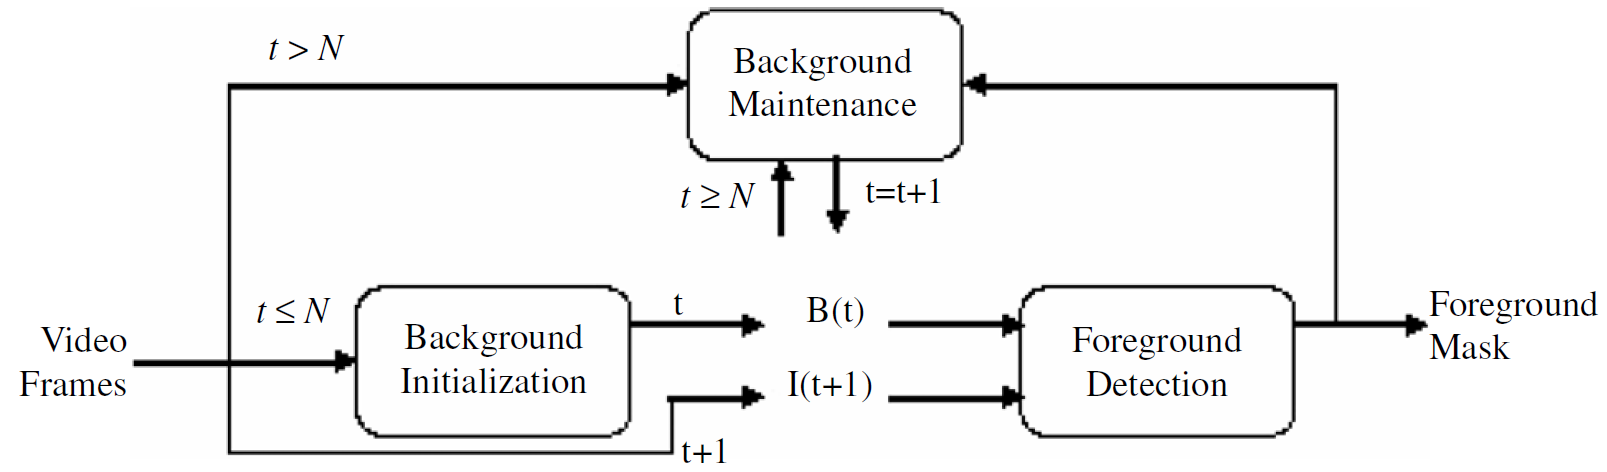
\includegraphics[width=0.85\textwidth]{img/chapters/estado-del-arte/background-subtraction-process.png}
\caption{\label{fig:background-subtraction-process}Proceso de la sustracción del fondo}
\end{figure}

A continuación se expone con más detalle cada una de las etapas que compone la sustracción del fondo:

\subsubsection*{Inicialización del fondo}
\label{subsubsec:inicializacion-del-fondo}

Modelado del fondo donde se describe el tipo de modelo que se esta utilizando para representar. Principalmente se determina la capacidad del modelo para trata con fondos estáticos (unimodal) o fondos dinámicos (multimodal).

En esta etapa se inicializa el modelo donde generalmente se utiliza el primer frame sobre un conjunto de frames de entrenamiento, los cuales contienen o no objetos en primer plano. El principal desafío es obtener un primer modelo de fondo cuando más de la mitad de los frames entrenamiento contiene objetos en primer plano.


\subsubsection*{Mantenimiento de fondo}
\label{subsubsec:mantenimiento-fondo}

El mantenimiento del fondo se encarga de adaptar el modelo a los cambios que puedan ser ocasionados a lo largo del tiempo. En esta etapa de aprendizaje se debe de realizar en línea por lo que el algoritmo debe de ser incremental. Los puntos claves en este proceso son los siguientes:

\begin{itemize}
    \item \textbf{Esquemas de mantenimiento}. En trabajos previos \cite{4712338} se presentan tres esquemas de mantenimientos: ciegos, selectivos y adaptativos difusos. El mantenimiento ciego del fondo actualiza todos los píxeles con las mismas reglas que se emplean en un filtro IIR:
    
    \begin{equation}
    \label{eq:IIR-filter}
    \text{B}_{t+1}(x,y) = (1 - \alpha)\text{B}_{t}(x,y) + \alpha\text{I}_{t}(x,y)
    \end{equation}
    
    donde:
    
    \begin{itemize}
        \item $\alpha$ es el ratio de aprendizaje y tiene un valor comprendido entre [0,1]
        \item $\text{B}_{t}$ y $\text{I}_{t}$ son el fondo y la imagen actual respectivamente en el tiempo t
    \end{itemize}
    
    La principal desventaja de este esquema es que el valor de los píxeles clasificados como primer plano son utilizados en el cálculo del nuevo fondo y por tanto, afecta a la imagen de fondo. Para lidiar con este problema algunos investigadores utilizan un esquema de mantenimiento selectivo que se basa en actualizar la nueva imagen de fondo con diferentes ratios de aprendizaje en función de la clasificación previa del píxel en primer plano o fondo:
    
    \vspace{0.5cm}

    $\text{B}_{t+1}(x,y) = (1 - \alpha)\text{B}_{t}(x,y) + \alpha\text{I}_{t}(x,y)$
    
    \vspace{0.5cm}
    
    si $(x,y)$ es el fondo
    
    \vspace{0.5cm}

    $\text{B}_{t+1}(x,y) = (1 - \beta)\text{B}_{t}(x,y) + \beta\text{I}_{t}(x,y)$
    
    \vspace{0.5cm}
    
    si $(x,y)$ es el primer plano
    
    \vspace{0.5cm}
    
    La idea es adaptar el píxel clasificado como fondo de manera rápida y un píxel clasificado como primer plano muy despacio. Por está razón $\beta \ll \alpha$ y generalmente $\beta = 0$. Por tanto, la ecuación \ref{eq:IIR-filter} se convierte en:
    
    \begin{equation}
    \label{eq:IIR-filter2}
    \text{B}_{t+1}(x,y) = \text{B}_{t}(x,y)
    \end{equation}
    
    El problema es que una clasificación errónea puede resultar un error permanente en el modelo del fondo. Este problema se puede solucionar mediante un esquema adaptativo difuso que toma en cuenta la incertidumbre de la clasificación. Esto puede lograrse graduando la regla de actualización utilizando el resultado de la detección del primer plano.
    
    \item \textbf{Ratio de aprendizaje}. Determina la velocidad de adaptación en los cambios de escena. Este ratio puede ser fijo, ajustado dinámicamente o difuso.
    \item \textbf{Mecanismos de mantenimiento}. El ratio de aprendizaje determina la velocidad de adaptación a los cambios de iluminación pero también el tiempo que necesita un cambio en el fondo hasta que se incorpora en el modelo, así como el tiempo donde un objeto que se encuentra en el primer plano estático puede sobrevivir antes de ser incluido en el modelo. El ratio de aprendizaje por tanto se encarga de diferentes desafíos diferenciados. Para desacoplar el mecanismo de adaptación y el de incorporación, \cite{1415580} utilizo un conjunto de contadores que representa el número de veces que un píxel se clasifica como píxel de primer plano. Cuando este número es mayor que cierto umbral, el píxel se considera que se encuentra en el fondo. Esto da un límite de tiempo de cuanto tiempo un píxel se encuentra en como píxel del primer plano estático.
    \item \textbf{Frecuencia de actualización}. El objetivo es actualizar el fondo solo cuando sea necesario. El mantenimiento se puede realizar en cada fotograma, sin embargo si no se producen cambios no es necesaria la actualización de los píxeles en cada frame.
\end{itemize}

\subsubsection*{Detección del primer plano}
\label{subsubsec:detección-primer-plano}

Esta etapa se trata de una tarea de clasificación que se encarga de etiquetar píxeles como fondo o como píxeles de primer plano.

\subsubsection*{Aplicaciones donde se utiliza la sustracción del fondo}
\label{subsubsec:aplicaciones-background-subtraction}

La segmentación de objetos en movimiento sobre el primer plano se utiliza en multitud de aplicaciones donde se emplea visión por computador como pueden ser:

\begin{itemize}
    \item \textbf{Videovigilancia inteligente}. Se trata de una de las aplicaciones donde más se utiliza esta metodología. El objetivo es detectar objetos en movimiento u objetos abandonados para garantizar la seguridad aérea, para calcular estadísticas de tráfico como se puede ver en la figura \ref{fig:background-subtraction-example} o para vigilancia marítima. Los objetos de interés suelen ser variados como vehículos, aviones, barcos, personas o equipajes.
    \item \textbf{Codificación de vídeo basada en el contenido}. Para generar un vídeo, debe de estar segmentado en objetos de vídeo y seguidos a medida que transcurren los frames del vídeo. El fondo y los objetos presentes en el vídeo son codificados por separado. En definitiva, la codificación en vídeo necesita métodos efectivos para la detección de objetos en entornos estáticos y dinámicos.
    \item \textbf{Captura de movimiento óptico}. El objetivo es obtener una captura completa y precisa de las personas mediante el uso de cámaras. La silueta se extrae generalmente en cada vista de la sustracción del fondo.
\end{itemize}

\begin{figure}[ht]
\centering
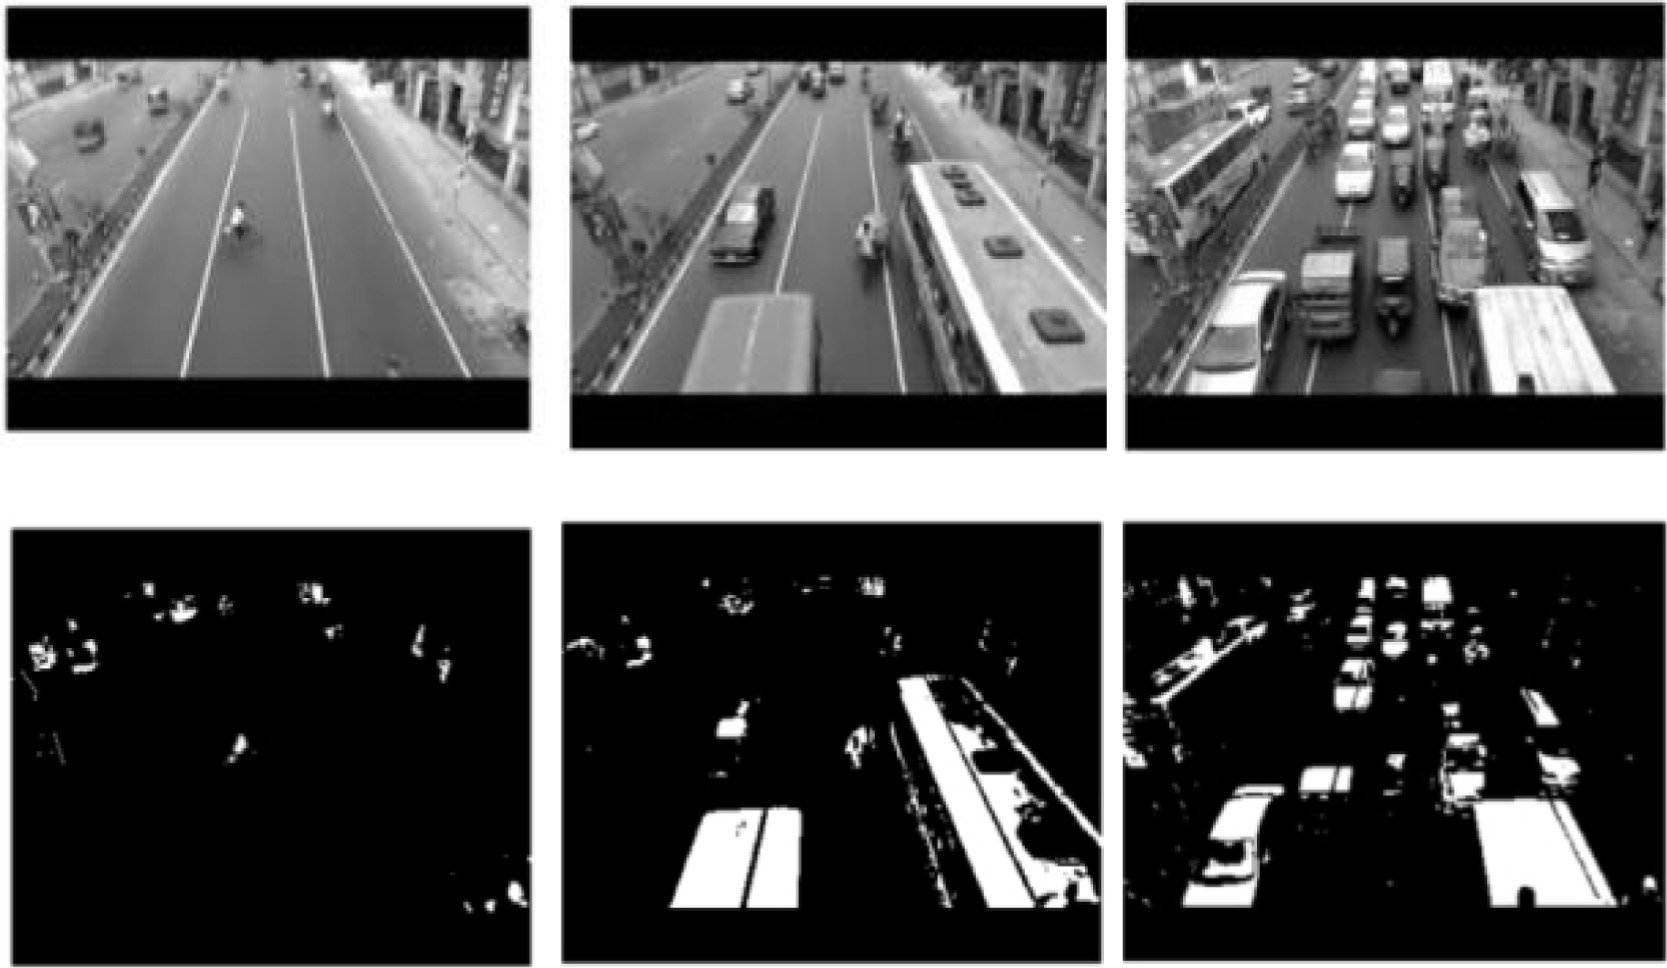
\includegraphics[width=0.75\textwidth]{img/chapters/estado-del-arte/background-subtraction-example.jpg}
\caption{\label{fig:background-subtraction-example}Ejemplo de sustracción del fondo en aplicaciones de tráfico}
\end{figure}



\subsection{Detección de objetos estacionarios}
\label{subsec:tecnicas-deteccion-obj-estacionarios}

La detección de objetos estacionarios está recibiendo una atención especial ya que se trata de una fase de análisis crítico en aplicaciones como la detección de objetos abandonados o vehículos estacionados en áreas públicas. El reconocimiento de objetos estacionarios en escenarios de grandes aglomeraciones de personas supone una tarea desafiante.

Se producen problemas ocasionados por las oclusiones o variación de colores y formas conforme las personas se mueven. Otros problemas que surgen son la iluminación, la velocidad de los objetos y la densidad de los objetos se deben de tener en cuenta. En la detección de objetos en primer planos, los métodos basados en la sustracción de fondo se han vuelto muy populares debido a que se suelen emplear cámaras fijas y los cambios de iluminación son muy graduales \cite{1217925}. En trabajos previos como en \cite{5279450} se propone enfoque en el análisis de imágenes estáticas.

En la figura \ref{fig:metodos-sustraccion-objeto-estacionario} se muestra clasificación de sustracción del fondo en base al método utilizado.

\begin{figure}[ht]
\centering
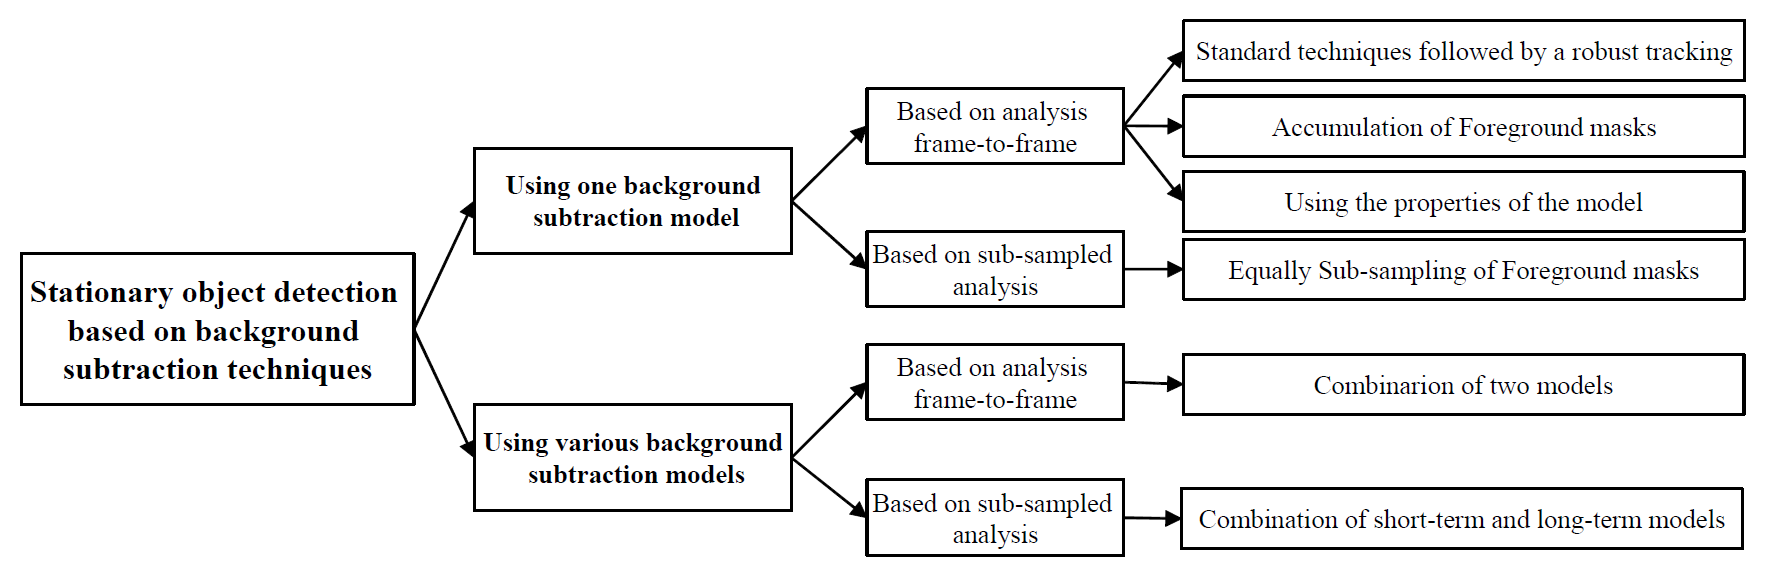
\includegraphics[width=1\textwidth]{img/chapters/estado-del-arte/metodos-sustraccion-fondo-deteccion-fondo-estacionario.png}
\caption{\label{fig:metodos-sustraccion-objeto-estacionario}Clasificación de sustracción del fondo basados en métodos de detección de objetos estacionarios}
\end{figure}

Dependiendo del uso de los mapas en primer plano calculados en el análisis de sustracción de fondo, los enfoques basados en un modelo se pueden clasificar en:

\begin{itemize}
    \item \textbf{Basado en análisis frame a frame}. Se emplean técnicas de sustracción del fondo seguidas de otro tipo análisis. En función de este tipo de análisis se puede clasificar en: basados en el uso de técnicas estándar de fondo seguido de otra etapa de análisis, basados en la acumulación de máscaras en primer plano calculadas frame a frame, o basado en las propiedades del modelo de sustracción de fondo utilizado.
    \item \textbf{Basado en análisis de submuestreo}. Estos propuestas tratan de detectar objetos estacionarios analizando las secuencias de vídeos a diferentes velocidades de frames. 
\end{itemize}

Los enfoques que combinan uno o más modelos de sustracción de fondo han sido menos estudiados. No obstante, una clasificación basada en el procesamiento de la velocidad de los frames se puede realizar de la siguiente manera:

\begin{itemize}
    \item \textbf{Basado en analisis frame a frame}. En esta categoría tenemos méotodso que combinan diferentes propiedades usando dos o varias técnicas sustracciones de fondo.
    \item \textbf{Basado en un análisis de submuestreo}. Estos enfoques detectan objetos estacionarios analizando las secuencias de vídeo con varios métodos de sustracción de fondo a diferentes velocidades de frames.
\end{itemize}

\subsection{Detección de personas y objetos}
\label{subsec:tecnicas-deteccion-personas-objetos}

Citar \cite{4657363}, y \cite{https://doi.org/10.1049/iet-cvi.2014.0148}

Y meter abstract + Architecture of people detection systems y Proposed classification of state-of-the-art
people detection de \cite{https://doi.org/10.1049/iet-cvi.2014.0148}

\textcolor{red}{La visión por computadora ha sido un campo en evolución durante los últimos años con múltiples líneas de investigación y diferentes dominios de aplicación. Video La vigilancia ha sido uno de los dominios más desarrollados para el últimos 10 años [1–4]. La necesidad de brindar seguridad a las personas y sus propiedades en todo el mundo explica el enorme desarrollo y expansión de los sistemas de videovigilancia en la actualidad. Video Los sistemas de vigilancia intentan extraer automáticamente información de la secuencia de vídeo y generar una descripción de la escena útil para interacciones humanas con el sistema: alarmas, registros, estadísticas, indexación y recuperación, etc. Dentro del campo de la visión por computador, particularmente en el área de investigación de procesamiento de imagen y video digital, existe una rica variedad de algoritmos para segmentación, detección de objetos, reconocimiento de eventos etc., que se utilizan en sistemas de vigilancia. Automático la detección de personas en secuencias de vídeo [5–8] es una de las más problemas desafiantes en la visión por computadora. La complejidad del El problema de detección de personas se basa principalmente en la dificultad de modelar a las personas debido a su gran variabilidad física apariencias, partes articuladas del cuerpo, poses, movimientos, puntos de vista e interacciones entre diferentes personas y objetos. Esta La complejidad es aún mayor en la vigilancia típica del mundo real. escenarios como aeropuertos, centros comerciales, etc., que a menudo incluyen múltiples personas, múltiples oclusiones y variabilidad de fondo.Hay una gran cantidad de encuestas de detección de personas en el literatura, algunos de ellos cubren parcialmente sólo el estado del arte o están claramente enfocados en alguna videovigilancia en particular solicitud. Enzweiler y Gavrila [5] presentan una encuesta de personas detección y también la integración de los detectores a bordo completo sistemas. Descompone los enfoques de detección de personas en tres Tareas de procesamiento: generación de hipótesis o regiones de objetos iniciales. de interés (ROI) selección, verificación (clasificación) y integración temporal (seguimiento). Gerónimo et al. [6] también presenta un Encuesta de detección de personas pero con un enfoque claro en el conductor. sistemas de asistencia y de una tubería de procesamiento: preprocesamiento, segmentación de primer plano, clasicación de objetos, verificación o perfeccionamiento, seguimiento y aplicación. Simonnet y col. [8] presenta una descripción general de los algoritmos de detección de personas centrados solo en enfoques de búsqueda exhaustivos, mientras que Dollár et al. [7] presentar una descripción general centrada únicamente en los enfoques de ventana deslizante. En este artículo, presentamos una clasificación de última generación que no centrado en una aplicación de videovigilancia en particular. Nosotros descomponer la detección de personas en subtareas, identificar los críticos tareas y clasificar el estado del arte de acuerdo con estas Tareas. De esta forma, podemos analizar las fortalezas y debilidades de cada enfoque de forma independiente y para cada crítico tarea. Cualquier otra subtarea adicional se considera un video específico. preprocesamiento o posprocesamiento de solicitudes de vigilancia y no forman parte del alcance de esta revisión. La principal contribución presentada en este documento es una descripción general y evaluación exhaustiva del estado del arte en detección de personas, en general, aplicaciones de videovigilancia. Por lo tanto, primero, los diferentes tareas de procesamiento que implican la detección automática de personas en Se han definido las secuencias de vídeo. Entonces, las tareas críticas tienen identi identcado y clasicaciones adecuadas de la detección de personas enfoques desde el estado de la técnica se han realizado de acuerdo con esas tareas críticas. Cada clasicación incluye una breve discusión sobre las ventajas y desventajas de los diferentes enfoques para Resuelve el problema de detección de personas en secuencias de video. Finalmente, Los experimentos se realizan sobre un extenso conjunto de datos con diferentes categorías de complejidad e incluyendo diferentes enfoques que cubre todos los problemas de detección de personas identicados en el estado del arte. El resto de este documento está estructurado de la siguiente manera: Sección 2 presenta una breve revisión del estado del arte, la Sección 3 describe la arquitectura básica de cada sistema de vigilancia por detector de personas,  La sección 4 presenta la clasificación propuesta de detección de personas estado de la técnica, las secciones 5 y 6 describen el rendimiento metodología de evaluación y resultados experimentales y, finalmente, la Las principales conclusiones se resumen en la Sección 7.}

\newpage

\subsection{Reconocimiento del comportamiento}
\label{subsec:tecnicas-reconocimiento-comportamiento}

Citar \cite{vishwakarma2012}, \cite{borges2013}, \cite{popoola2012} y \cite{BENMABROUK2018480}

Meter abstract + Classifying abnormal behavior recognition methods de \cite{BENMABROUK2018480}

\textcolor{red}{El reconocimiento de la acción humana en los videos es un campo activo en la visión por computadora que está atrayendo más atención de la investigación en los últimos años. Este tema se vuelve muy importante para muchas aplicaciones como la videovigilancia, el modelado de escenas y la anotación y recuperación de contenido de video. Varias encuestas anteriores sobre detección y análisis de movimiento humano (Aggarwal y Cai, 1999, 1997; Ji y Liu, 2010), análisis y comprensión del comportamiento (Pantic, Pentland, Nijholt y Huang, 2007; Teddy, 2008) y reconocimiento de actividades (Shian -Ru et al., 2013) (Tabla 1). Recientemente, Dawn, Debapratim, Shaikh y SoharabHossain (2015) y Hassan et al. (2014) revisaron varios métodos basados en técnicas de visión por computadora para reconocer actividades simples realizadas por una sola persona como correr y caminar. Bux, Plamen y Zulfiqar (2017) revisaron técnicas relativas a las diferentes fases del reconocimiento de la actividad humana, que son la segmentación de objetos, la extracción y representación de características y la clasificación de actividades. En particular, Sarvesh y Anupam (2013) y Mishra y Bhagat (2015) presentaron técnicas para el análisis de movimiento y el reconocimiento de actividad en aplicaciones de videovigilancia. De hecho, la detección de un comportamiento anormal en la videovigilancia es esencial para garantizar la seguridad tanto en lugares interiores como exteriores, como estaciones de tren y aeropuertos. De hecho, la detección de conductas anormales es un problema particular del reconocimiento de la acción humana. Con el creciente número de cámaras de vigilancia, la tarea de supervisar múltiples monitores por parte de los agentes de seguridad se vuelve muy difícil debido a la falta de atención y la fatiga humana. Además, los eventos anormales son relativamente raros y no ocurren con frecuencia. Esto hace que la tarea de supervisión sea más compleja y desafiante. Por tanto, existe una demanda creciente de un sistema de videovigilancia inteligente que detecte, automáticamente, un comportamiento anormal y emita una alarma. De hecho, se proporcionaron encuestas anteriores de sistemas de videovigilancia. Por ejemplo, Valera y Velastin (2005) presentaron una descripción general de los sistemas de vigilancia automatizados para la detección de anomalías. Oluwatoyin y Kejun (2012) proporcionaron una encuesta de métodos de comportamiento humano anormal en aplicaciones de videovigilancia en diferentes contextos. Más recientemente, Zablocki, K., D. y R. (2014) revisaron diferentes técnicas utilizadas por los sistemas de vigilancia inteligente para monitorear los espacios públicos. Los métodos de detección de eventos anormales en los videos de vigilancia de multitudes fueron analizados por de Campos (2014) y Teng et al. (2015). En este artículo, revisamos ampliamente los métodos existentes que se utilizan en aplicaciones de videovigilancia y destacamos los avances actuales en el campo de la detección de comportamientos anormales. El objetivo de un sistema de videovigilancia inteligente es detectar de manera eficiente un evento interesante a partir de una gran cantidad de videos para prevenir situaciones peligrosas. Generalmente, esta tarea requiere dos niveles de procesamiento de video como se muestra en la Fig.1. El primero consta de dos pasos. Primero, se extraen características de bajo nivel, con el objetivo de detectar la región de interés en la escena. Luego, se generan primitivas basadas en características de bajo nivel para describir la región de interés. El segundo nivel proporciona información semántica sobre la acción humana y determina si el comportamiento es normal o no. El resto de este documento está organizado de la siguiente manera. En la Sección 2, se presentan las técnicas más importantes para la representación del comportamiento, incluida la extracción y descripción de características. En la Sección 3 se revisan los diferentes marcos y métodos de clasificación para el modelado del comportamiento, tanto en escenas con mucha gente como con poca gente. En la Sección 4, se presentan por primera vez los conjuntos de datos más populares utilizados para evaluar un sistema de videovigilancia. Luego, se proporciona una evaluación de desempeño de trabajos anteriores. En la Sección 5 se describen ejemplos de sistemas de videovigilancia existentes en el mundo real. Finalmente, en la Sección 6 se proporciona una conclusión y una discusión de esta revisión.}

\newpage

\section{Redes neuronales convolucionales (CNN)}
\label{sec:intro-redes-neuronales-convolucionales}

Las redes neuronales convolucionales (\gls{cnn}) son un subconjunto de algoritmos de \textit{Deep Learning} de aprendizaje tanto supervisado, como por ejemplo en la clasificación de imágenes, y no supervisado como puede ser la incrustación de palabras. Las \gls{cnn} son un tipo de red neuronal artificial que se utiliza en el análisis de datos con estructura similar a una cuadrícula. Un ejemplo buen ejemplo son los datos de imágenes que pueden ser represententados en dos dimensiones con valores \gls{rgb}. En problemas como pueden ser la clasificación imágenes, hay tres principales desafíos donde se usan \gls{mlp} los cuales las \gls{cnn} pueden resolver:

\begin{figure}[ht]
\centering
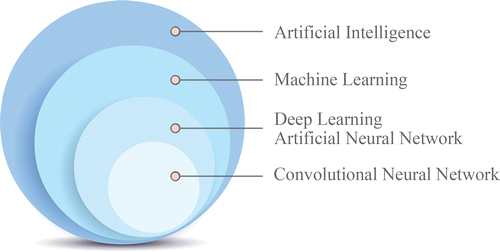
\includegraphics[width=0.45\textwidth]{img/chapters/estado-del-arte/cnn-radiologic.png}
\caption{\label{fig:cnn-dlnn}Las CNN son un subconjunto de redes neuronales de Deep Learning}
\end{figure}

\begin{itemize}
    \item \textbf{Crecimiento de parámetros}. El uso de un perceptron por cada píxel hace que la cantidad de parámetros aumente rápidamente.
    \item \textbf{Traducciones}. Un \gls{mlp} estándar trataría una imagen y su versión ligeramente desplaza como dos imágenes complemente diferentes. Por ejemplo, reconocer un automóvil en una imagen no debería de depender de en que lugar de la imagen se encuentra.
    \item \textbf{Espacialidad}. Los \gls{mlp} no tienen en cuenta las relaciones espaciales en las imágenes. El hecho de que dos píxeles se encuentren cerca es información significativa.
\end{itemize}

Las \gls{cnn} resuelven el problema de la comprensión de las imágenes, utilizando con mayor facilidad redes complejidad. La red neurona especial tiene en cuenta que la cercanía entre píxeles tiene significado y que los elementos de interés pueden aparecer en cualquier parte de una imagen. Esto se logra mediante el uso de una operación de convolución lineal. El uso de esta operación en una o mas capas es lo que define a una \gls{cnn}. En ocasiones las suposiciones subyacentes a las opciones de diseño de las \gls{cnn} deben disminuirse o alterarse debido a la naturaleza de los datos de entrada. Aunque la complejidad computacional es más manejable, las redes tienden a ser más profundas. Esto crea algoritmos inteligentes para calcular las convoluciones.

\begin{figure}[ht]
\centering
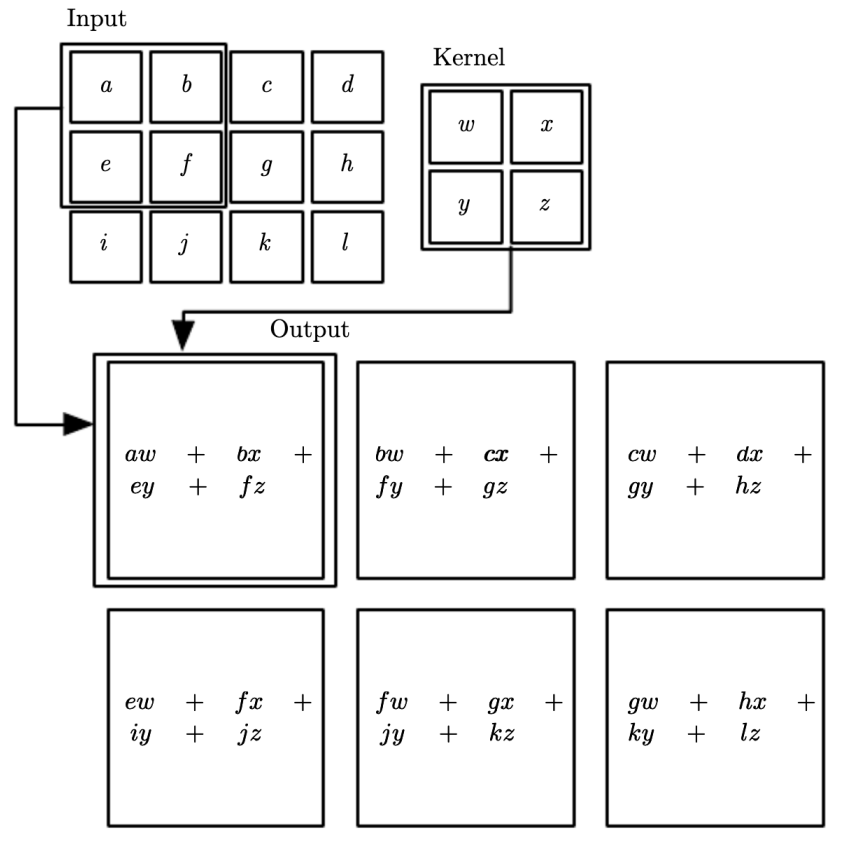
\includegraphics[width=0.3\textwidth]{img/chapters/estado-del-arte/ejemplo-convolucion.png}
\caption{\label{fig:ejemplo-convolucion}Ejemplo de convolución de datos de entrada bidimensionales}
\end{figure}

La idea principal detrás de la convolución es la identificación de características en los datos de entrada mediante la aplicación de un kernel (también conocido como filtro) en los datos de entrada. Tanto los datos de entrada como el kernel tienen una estructura similar a una cuadrícula y se pueden representar como tensores, que son matrices multidimensionales. El kernel puede ser de cualquier tamaño y, por lo general, es más pequeño que los datos de entrada. Los núcleos se utilizan para identificar características en los datos de entrada, como los bordes de una imagen. Los datos de entrada se convolucionan con el kernel, lo que significa que el kernel se "desliza" a través de los datos de entrada, calculando el producto escalar o el producto matricial (según las dimensiones) entre la parte superpuesta de los datos de entrada y el kernel. En la figura \ref{fig:ejemplo-convolucion} se puede ver un ejemplo ilustrativo de la operación de convolución.

La operación de convolución se define como:

\begin{equation}
\label{eq:operacion-convolucion1}
s(t) = (x*w)(t) = \int x(a)w(t-a)da
\end{equation}

donde $x$ es la función que se asigna a un valor específico en los datos de entrada y $w$ representa el núcleo. Esta formulación se puede considerar como un promedio de suavizado de $x$ en todo su dominio, dando mayor peso a los valores más cercanos a $t$. Si los valores de entrada son discretos, la operación de convolución se puede reescribir mediante la suma:

\begin{equation}
\label{eq:operacion-convolucion2}
s(t) = (x*w)(t) = \sum_{a=-\infty}^\infty x(a)w(t-a)
\end{equation}

La entrada suele ser multidimensional. En ese caso, se pueden reemplazar las funciones con funciones multivariables, es decir, operando en tensores. Suponiendo un ejemplo de aplicación de convolución a una imagen bidimensional $I$ como entrada. Luego, se puede usar un kernel $K$ bidimensional, y la operación se puede escribir de la siguiente manera:

\begin{equation}
\label{eq:operacion-convolucion3}
S(i,j) = (I*K)(i,j) = \sum_{m} \sum_{n} I(m,n) K (i - m, j - n)
\end{equation}

Es decir, dado un píxel en la entrada, ubicado en la fila $i$ y la columna $j$, la convolución se calcula colocando el centro del núcleo sobre el píxel de entrada y sumando el producto de los parámetros del núcleo superpuestos y los píxeles de entrada para producir el valor de salida para $i$ y $j$.

\subsection*{Ejemplo de aplicación: Detección de tumores en mamografías}
\label{subsec:ejemplos-aplicacion-cnn}

Una aplicación interesante de las redes neuronales convolucionales se encuentra dentro del campo de la radiología. Cada año, millones de mujeres se someten a un tratamiento para la detección de cánceres en una etapa temprana mediante mamografías. El artículo \cite{mammography2019} muestra que las \gls{cnn} ya pueden detectar cánceres en una etapa temprana con alta precisión. De hecho, su algoritmo ya está superando en muchos aspectos a los médicos estadounidenses. El uso de \gls{cnn} en el diagnóstico puede reducir en gran medida el costo para los hospitales, haciendo que las pruebas estén disponibles para un público más amplio y, al mismo tiempo, aumentando la precisión del diagnóstico.

\begin{figure}[ht]
\centering
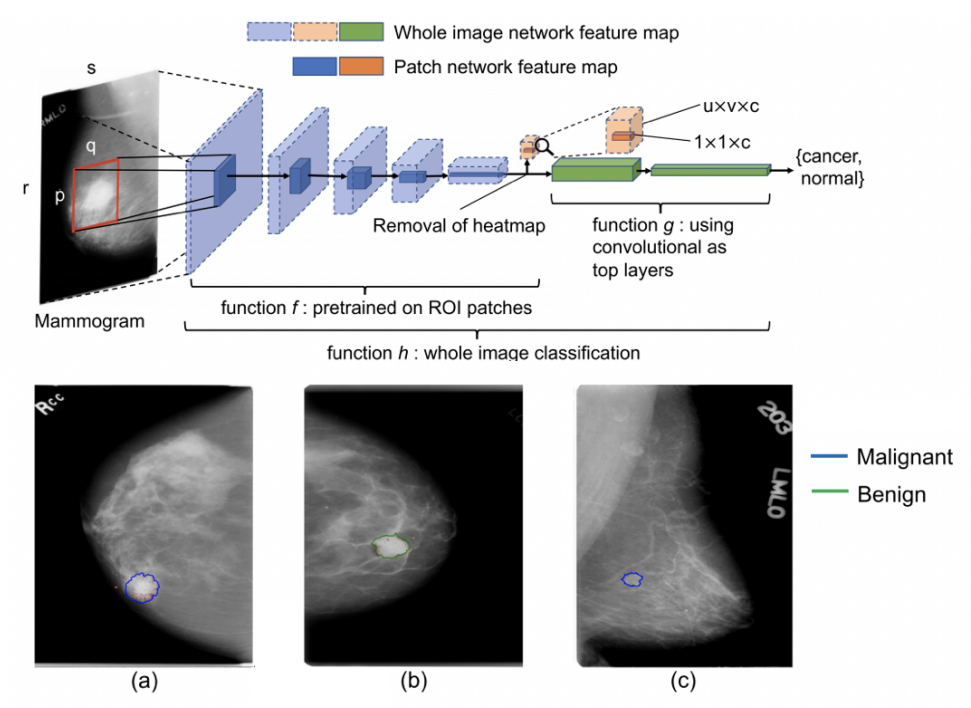
\includegraphics[width=0.5\textwidth]{img/chapters/estado-del-arte/cnn-mamografia.png}
\caption{\label{fig:ejemplo-mamografia}Ejemplo de convolución de datos de entrada bidimensionales}
\end{figure}

La CNN resultante se ejecutó en varias bases de datos con un \gls{auc} en las imágenes de menor calidad de 0,91. Entrenando una red con imágenes de alta resolución de la base de datos INbreast \cite{moreira2011}, su mejor modelo logró un \gls{auc} por imagen de 0,95. Combinando todos sus modelos, este número se elevó hasta 0,98 con una sensibilidad del 86,7\% y una especificidad del 96,1\%. Esto muestra que las \gls{cnn} pueden realizar tareas que ahorran costos pero, lo que es más importante, salvan vidas. Con el resultado del artículo \cite{mammography2019}, esto significaría que la \gls{cnn} está superando al personal médico en la detección y clasificación de tumores. Los médicos tienen solo un 0,3\% más de probabilidades de detectar correctamente un tumor maligno, pero tienen un 7,2\% menos de probabilidades de encontrar correctamente que un paciente esté sano.

\section{Algoritmos de detección de objetos}
\label{sec:tecnicas-utilizadas-detection}

\subsection{Faster R-CNN}
\label{subsec:faster-rcnn}

Faster \gls{r-cnn} es una extensión de Fast \gls{r-cnn} \cite{7410526}. Como su nombre indica, Faster \gls{r-cnn} es más rápido que Fast \gls{r-cnn} gracias a la red de propuesta regional (\gls{rpn}).

La arquitectura de Faster \gls{r-cnn} se muestra en la siguiente figura. Consta de 2 módulos:

\begin{itemize}
    \item \gls{rpn}: para generar propuestas regionales.
    \item Fast \gls{r-cnn}: para detectar objetos en las regiones propuestas.
\end{itemize}

El módulo \gls{rpn} es responsable de generar propuestas regionales. Aplica el concepto de atención en redes neuronales, por lo que guía al módulo de detección Fast \gls{r-cnn} hacia dónde buscar objetos en la imagen.

\begin{figure}[ht]
\centering
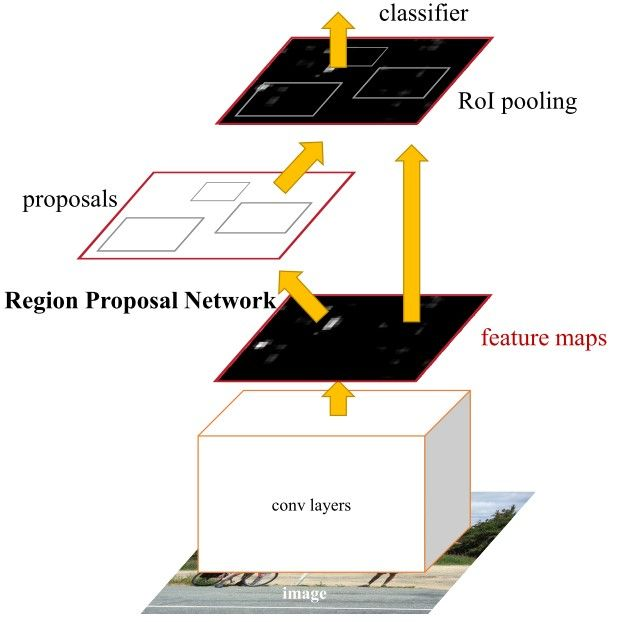
\includegraphics[width=0.45\textwidth]{img/chapters/estado-del-arte/arquitectura-faster-rcnn.jpg}
\caption{\label{fig:arquitectura-faster-rcnn}Arquitectura de Faster R-CNN}
\end{figure}

Las capas convolucionales se comparten entre los módulos \gls{rpn} y Fast \gls{r-cnn}.

Faster R-CNN funciona de la siguiente manera:

\begin{itemize}
    \item El \gls{rpn} genera propuestas regionales.
    \item Para todas las propuestas de región en la imagen, se extrae un vector de características de longitud fija de cada región utilizando la capa de agrupación de \gls{roi}.
    \item Los vectores de características extraídos luego se clasifican usando Fast \gls{r-cnn}.
    \item Se devuelven las puntuaciones de clase de los objetos detectados además de sus cuadros delimitadores.
\end{itemize}

\subsubsection*{Region Proposal Network (RPN)}
\label{subsubsec:region-proposal-network}

Los modelos \gls{r-cnn} y Fast \gls{r-cnn} dependen del algoritmo de búsqueda selectiva para generar propuestas de región. Cada propuesta se envía a una \gls{cnn} previamente capacitada para su clasificación. En \cite{ren2016faster} se propuso una red denominada red de propuestas regionales (\gls{rpn}) que puede producir las propuestas regionales. Esto tiene algunas ventajas:

\begin{enumerate}
    \item Las propuestas de región ahora se generan utilizando una red que podría entrenarse y personalizarse de acuerdo con la tarea de detección.
    \item Debido a que las propuestas se generan utilizando una red, esta se puede entrenar de un extremo a otro para personalizarla en la tarea de detección. Por lo tanto, produce mejores propuestas de región en comparación con métodos genéricos como Selective Search y EdgeBoxes.
    \item El \gls{rpn} procesa la imagen utilizando las mismas capas convolucionales utilizadas en la red de detección Fast \gls{r-cnn}. Por lo tanto, el \gls{rpn} no necesita más tiempo para producir las propuestas en comparación con los algoritmos como la búsqueda selectiva.
    \item Debido a que comparten las mismas capas convolucionales, el \gls{rpn} y el Fast \gls{r-cnn} se pueden fusionar/unificar en una sola red. Por lo tanto, el entrenamiento se realiza solo una vez.
\end{enumerate}

El \gls{rpn} funciona en el mapa de características de salida devuelto desde la última capa convolucional compartida con Fast \gls{r-cnn}. Esto se muestra en la siguiente figura. Sobre la base de una ventana rectangular de tamaño $n*n$, una ventana deslizante atraviesa el mapa de características. Para cada ventana, se generan varias propuestas de regiones candidatas. Estas propuestas no son las propuestas finales, ya que se filtrarán en función de su ``puntuación de objetividad''.

\subsubsection*{Anchor}
\label{subsubsec:anchor-faster-rcnn}

Como se puede ver en la figura \ref{fig:variacion-anchor-boxes-faster-rcnn}, el mapa de características de la última capa de convolución compartida se pasa a través de una ventana deslizante rectangular de tamaño $n*n$, donde $n = 3$ para la red VGG-16. Para cada ventana, se generan propuestas de región $K$. Cada propuesta se parametriza según un cuadro de referencia que se denomina \textit{anchor box}. Los 2 parámetros de los anchor boxes son:

\begin{enumerate}
    \item Escala
    \item Relación de aspecto
\end{enumerate}

Generalmente, hay 3 escalas y 3 relaciones de aspecto y, por lo tanto, hay un total de $K = 9$ casillas de anclaje. Pero $K$ puede ser diferente de 9. En otras palabras, $K$ regiones se producen a partir de cada propuesta de región, donde cada una de las $K$ regiones varía en la escala o en la relación de aspecto. Algunas de las variaciones del ancla se muestran en la figura \ref{fig:variacion-anchor-boxes-faster-rcnn}.

\begin{figure}[ht]
\centering
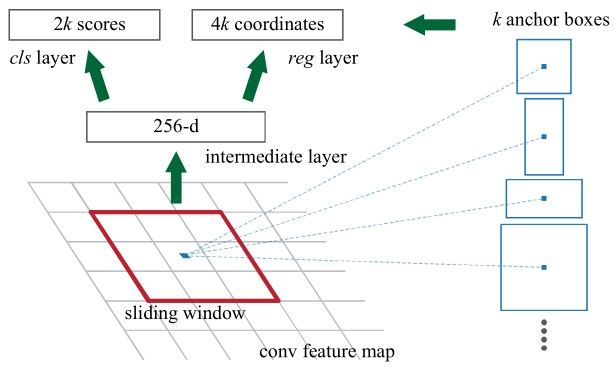
\includegraphics[width=0.45\textwidth]{img/chapters/estado-del-arte/variacion-anchor-boxes-faster-rcnn.jpg}
\caption{\label{fig:variacion-anchor-boxes-faster-rcnn}Variación de los anchor boxes Faster R-CNN}
\end{figure}

Utilizando anclajes de referencia (anchor boxes), se utiliza una sola imagen a una sola escala y, al mismo tiempo, se pueden ofrecer detectores de objetos invariantes en escala, ya que los anclajes existen a diferentes escalas. Esto evita el uso de múltiples imágenes o filtros. Los anclajes de múltiples escalas son clave para compartir características en el \gls{rpn} y la red de detección Fast \gls{r-cnn}.

Para cada propuesta de región $n*n$, se extrae un vector de características (de longitud 256 para la red ZF y 512 para la red VGG-16). Este vector luego se alimenta a 2 capas hermanas completamente conectadas:

\begin{enumerate}
    \item La primera capa \gls{fc} se llama \texttt{cls} y representa un clasificador binario que genera la puntuación de objetividad para cada propuesta de región (es decir, si la región contiene un objeto o es parte del fondo).
    \item La segunda capa \gls{fc} se llama \texttt{reg}, que devuelve un vector 4-D que define el cuadro delimitador de la región.
\end{enumerate}

La primera capa \gls{fc} (es decir, clasificador binario) tiene 2 salidas. El primero es para clasificar la región como fondo y el segundo es para clasificar la región como un objeto. La siguiente sección analiza cómo se asigna la puntuación de objetividad a cada ancla y cómo se utiliza para producir la etiqueta de clasificación.

\subsection{SSD: Single Shot MultiBox Detector}
\label{subsec:ssd}

\gls{ssd} es un moldeo de detección de objetos en imágenes empleando únicamente una \gls{dnn}. \gls{ssd} discretiza el espacio de salida de los cuadros delimitadores en un conjunto de cuadros predeterminados en diferentes proporciones y escalas por ubicación del mapa de características. En el momento de la predicción, la red genera puntuaciones para la presencia de cada categoría de objeto en cada cuadro predeterminado y produce ajustes en el cuadro para que coincida mejor con la forma del objeto. Además, la red combina predicciones de múltiples mapas de características con diferentes resoluciones para manejar de forma natural objetos de varios tamaños.

\gls{ssd} tiene dos componentes: un modelo backbone y un \gls{ssd} head. El modelo backbone suele ser una red de clasificación de imágenes previamente entrenadas como extractor de características. Típicamente suele ser una red como \texttt{ResNet} entrenada en ImageNet \cite{russakovsky2015imagenet} de la que se ha eliminado la capa de clasificación final completamente conectada. Por tanto, nos quedamos con una \gls{dnn} que es capaz de extraer el significado semántico de la imagen de entrada al tiempo que conserva la estructura espacial de la imagen, aunque con una resolución más baja. Para \texttt{ResNet34}, el backbone da como resultado un mapa de características de 256 7x7 para una imagen de entrada. El \gls{ssd} head es solo una o más capas convolucionales agregadas a este backbone y las salidas se interpretan como los cuadros delimitadores y las clases de objetos en la ubicación espacial de las activaciones de las capas finales.

En la figura \ref{fig:ssd-structure}, las primeras capas (cuadros blancos) son el backbone, las últimas capas (cuadros azules) representan el SSD head.


\begin{figure}[ht]
\centering
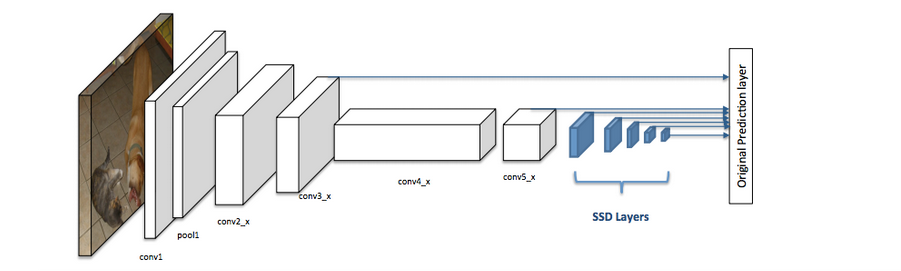
\includegraphics[width=1\textwidth]{img/chapters/estado-del-arte/ssd-structure.png}
\caption{\label{fig:ssd-structure}Arquitectura de una red neuronal convolucional con un detector SSD}
\end{figure}

\subsubsection*{Grid cell}
\label{subsubsec:grid-cell-ssd}

En lugar de usar una ventana deslizante, \gls{ssd} divide la imagen usando una cuadrícula y cada celda de la cuadrícula es responsable de detectar objetos en esa región de la imagen. La detección de objetos simplemente significa predecir la clase y ubicación de un objeto dentro de esa región. Si no hay ningún objeto presente, se considera como la clase de fondo y se ignora la ubicación. Por ejemplo, como se puede observar en la figura usar una cuadrícula de 4x4 en el siguiente ejemplo. Cada celda de la cuadrícula puede mostrar la posición y la forma del objeto que contiene.

\begin{figure}[ht]
\centering
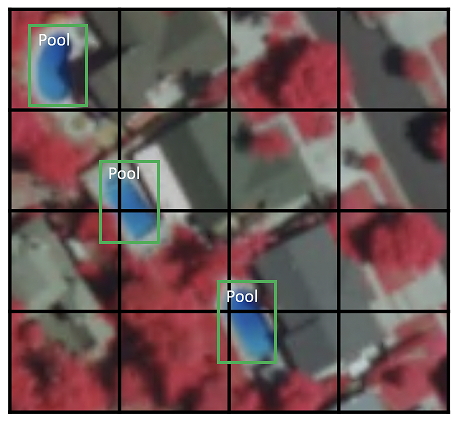
\includegraphics[width=0.35\textwidth]{img/chapters/estado-del-arte/gridcell.png}
\caption{\label{fig:ejemplo-grid-cell}Ejemplo de una cuadrícula 4x4}
\end{figure}

\subsubsection*{Anchor box}
\label{subsubsec:anchor-box-ssd}

Cada grid cell en \gls{ssd} se puede asignar con múltiples anchor boxes. Estos anchor boxes están predefinidos y cada uno es responsable de un tamaño y forma dentro de una grid cell. Por ejemplo, la piscina de la imagen siguiente corresponde a la anchor box más alta, mientras que el edificio corresponde a la anchor box más ancha.

\begin{figure}[ht]
\centering
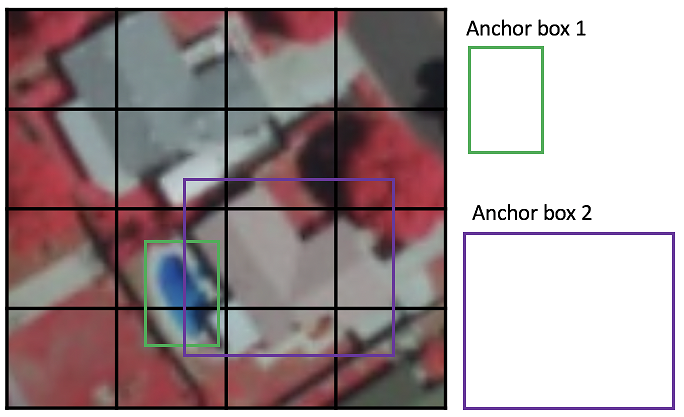
\includegraphics[width=0.45\textwidth]{img/chapters/estado-del-arte/ejemplo-2-anchor-boxes.png}
\caption{\label{fig:ejemplo-2-anchor-boxes}Ejemplo con 2 anchor boxes}
\end{figure}

\gls{ssd} usa una fase de coincidencia durante el entrenamiento, para hacer coincidir el anchor box apropiado con los cuadros delimitadores de cada objeto de ground truth dentro de una imagen. Básicamente, el anchor box con el mayor grado de superposición con un objeto es responsable de predecir la clase de ese objeto y su ubicación. Esta propiedad se utiliza para entrenar la red y para predecir los objetos detectados y sus ubicaciones una vez que la red ha sido entrenada. En la práctica, cada anchor box se especifica mediante una relación de aspecto y un nivel de zoom.

\subsubsection*{Relación de aspecto}
\label{subsubsec:aspect-ratio-ssd}

No todos los objetos tienen forma cuadrada. Algunos son más largos y otros más anchos, en diversos grados. La arquitectura \gls{ssd} permite relaciones de aspecto predefinidas de los anchor boxes para tener en cuenta esto. El parámetro de proporciones se puede utilizar para especificar las diferentes proporciones de los cuadros de anclaje asociados con cada celda de la cuadrícula en cada nivel de zoom/escala.

\begin{figure}[ht]
\centering
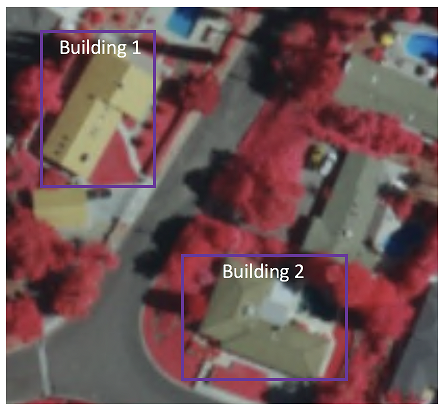
\includegraphics[width=0.35\textwidth]{img/chapters/estado-del-arte/aspect_ratio-ejemplo-ssd.png}
\caption{\label{fig:aspect_ratio-ejemplo-ssd}El cuadro delimitador del edificio 1 es más alto, mientras que el cuadro delimitador del edificio 2 es más ancho}
\end{figure}

\subsubsection*{Nivel de zoom}
\label{subsubsec:zoom-level-ssd}

No es necesario que los anchor boxes tengan el mismo tamaño que grid cell. Podríamos estar interesados en encontrar objetos más pequeños o más grandes dentro de una celda de la cuadrícula. El parámetro de zoom se utiliza para especificar cuánto deben ampliarse o reducirse los cuadros de anclaje con respecto a cada celda de la cuadrícula. Al igual que lo que hemos visto en el ejemplo de el anchor box, el tamaño del edificio es generalmente más grande que la piscina.

\subsubsection*{Campo receptivo}
\label{subsubsec:receptive-field-ssd}

El campo receptivo se define como la región en el espacio de entrada que está mirando una función de \gls{cnn} en particular, es decir, que se ve afectada. Debido a la operación de convolución, las características en diferentes capas representan diferentes tamaños de región en la imagen de entrada. A medida que se profundiza, el tamaño representado por una característica aumenta. En este ejemplo que se puede observar en la figura \ref{fig:receptive-field-ssd}, se comienza con la capa inferior (5x5) y luego se aplica una convolución que da como resultado la capa intermedia (3x3) donde una característica (píxel verde) representa una región de 3x3 de la capa de entrada (capa inferior). Y luego se aplica la convolución a la capa intermedia y se obtiene la capa superior (2x2) donde cada característica corresponde a una región de 7x7 en la imagen de entrada. Este tipo de matriz 2D verde y naranja también se denomina mapas de características, que se refieren a un conjunto de características creadas al aplicar el mismo extractor de características en diferentes ubicaciones del mapa de entrada en una ventana deslizante. Las características del mismo mapa de características tienen el mismo campo receptivo y buscan el mismo patrón pero en diferentes ubicaciones. Esto crea la invariancia espacial de \texttt{ConvNet}.

\begin{figure}[ht]
\centering
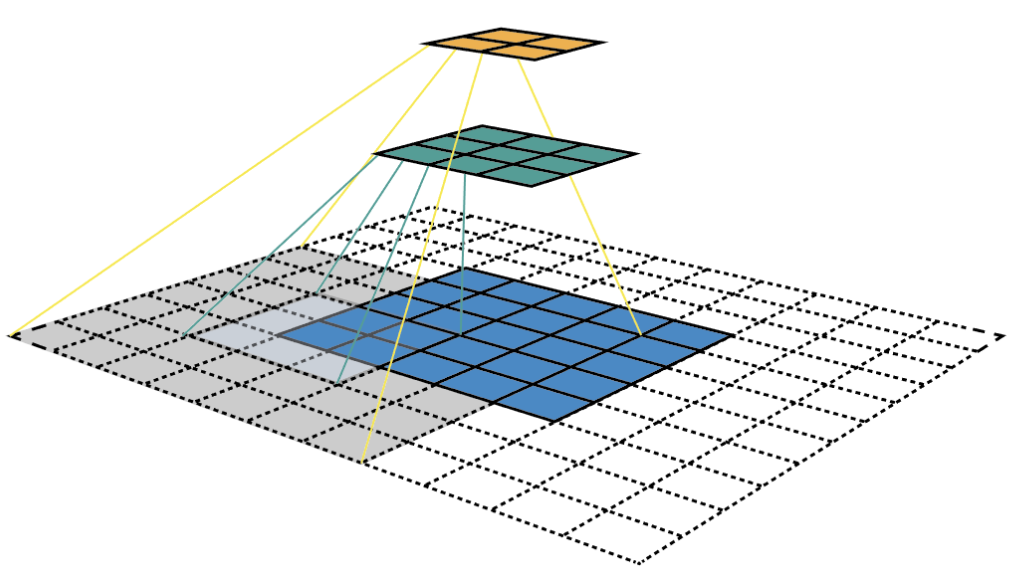
\includegraphics[width=0.45\textwidth]{img/chapters/estado-del-arte/receptive-field.png}
\caption{\label{fig:receptive-field-ssd}Visualización de mapas de características de CNN y campo receptivo}
\end{figure}

El campo receptivo es la premisa central de la arquitectura SSD, ya que permite detectar objetos a diferentes escalas y generar un cuadro delimitador más ajustado. el backbone ResNet34 genera mapas de características de 256 7x7 para una imagen de entrada. Si especificamos una cuadrícula de 4x4, el enfoque más simple es simplemente aplicar una convolución a este mapa de características y convertirlo a 4x4. Este enfoque puede funcionar hasta cierto punto y es exactamente la idea de \gls{yolo}. El paso extra dado por \gls{ssd} es que aplica más capas convolucionales al mapa de características del backbone y hace que cada una de estas capas de convolución genere resultados de detección de objetos. Como las capas anteriores que tienen un campo receptivo más pequeño pueden representar objetos de menor tamaño, las predicciones de las capas anteriores ayudan a tratar con objetos de menor tamaño.

Debido a esto, \gls{ssd} permite definir una jerarquía de celdas de cuadrícula en diferentes capas. Por ejemplo, se podría usar una cuadrícula de 4x4 para encontrar objetos más pequeños, una cuadrícula de 2x2 para encontrar objetos de tamaño medio y una cuadrícula de 1x1 para encontrar objetos que cubran toda la imagen.

\subsection{EfficientDet}
\label{subsec:efficientdet}

EfficientDet se trata de un detector de objetos escalables y eficientes. Sobre la base de nuestro trabajo anterior sobre el escalado de redes neuronales que logra una alta precisión y es hasta 9 veces más pequeño y usa significativamente menos cálculos en comparación con los detectores del Estado del Arte. En la figura \ref{fig:arquitectura-efficientdet} se muestra la arquitectura de red general de nuestros modelos.

\begin{figure}[ht]
\centering
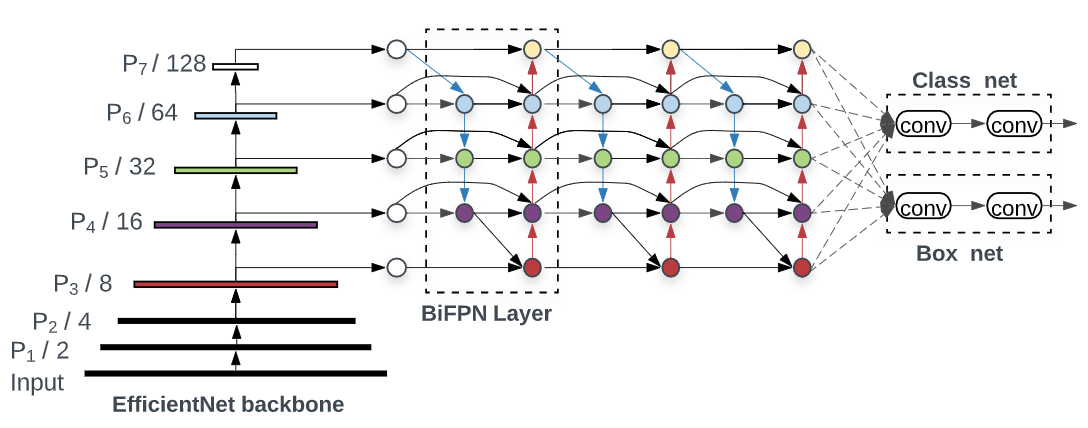
\includegraphics[width=0.8\textwidth]{img/chapters/estado-del-arte/arquitectura-efficientdet.png}
\caption{\label{fig:arquitectura-efficientdet}Arquitectura de EfficientDet}
\end{figure}

EfficientDet surge en noviembre de 2019 con la necesidad de aplicar soluciones en la mejora de la eficiencia computacional mediante la realización de un estudio sistemático de modelos de detección de última generación. Como ya se vió en la sección \ref{subsec:ssd}, los detectores de objetos tienen tres componentes principales: un backbone que extrae características de la imagen dada, una red de características que toma múltiples niveles de características de la red troncal como entrada y genera una lista de características fusionadas que representan características de la imagen y una red final que usa las características fusionadas para predecir la clase y ubicación de cada objeto. Al examinar las opciones de diseño para estos componentes, EfficientDet identifica varias optimizaciones clave para mejorar el rendimiento y la eficiencia.

Los detectores de objetos anteriores se basan principalmente en ResNets, ResNeXt o AmoebaNet como backbones, que son menos potentes o tienen menor eficiencia que la de EfficientNet. Al implementar primero un backbone EfficientNet, es posible lograr una eficiencia mucho mayor. Por ejemplo, a partir de una RetinaNet que emplea el backbone ResNet-50, se puede observar que simplemente reemplazar ResNet-50 con EfficientNet-B3 puede mejorar la precisión en un 3\% y reducir los cálculos en un 20\%.

Otra optimización es mejorar la eficiencia de las redes de características. Si bien la mayoría de los detectores anteriores simplemente emplean una \gls{fpn}, se puede observar que el \gls{fpn} de arriba hacia abajo está inherentemente limitado por el flujo de información unidireccional. Los \gls{fpn} alternativos, como PANet, agregan un flujo ascendente adicional a costa de más cálculos. Los esfuerzos para aprovechar la \gls{nas} descubrieron la arquitectura \gls{nas}-\gls{fpn} más compleja. Sin embargo, si bien esta estructura de red es efectiva, también es irregular y altamente optimizada para una tarea específica, lo que dificulta la adaptación a otras tareas.

Para abordar estos problemas, EfficientDet presenta una nueva red de funciones bidireccionales, Bi\gls{fpn}, que incorpora la idea de fusión de funciones multinivel de \gls{fpn}/PANet /\gls{nas}-\gls{fpn} que permite que la información fluya tanto en la dirección de arriba hacia abajo como de abajo hacia arriba, mientras utiliza conexiones regulares y eficientes.

\begin{figure}[ht]
\centering
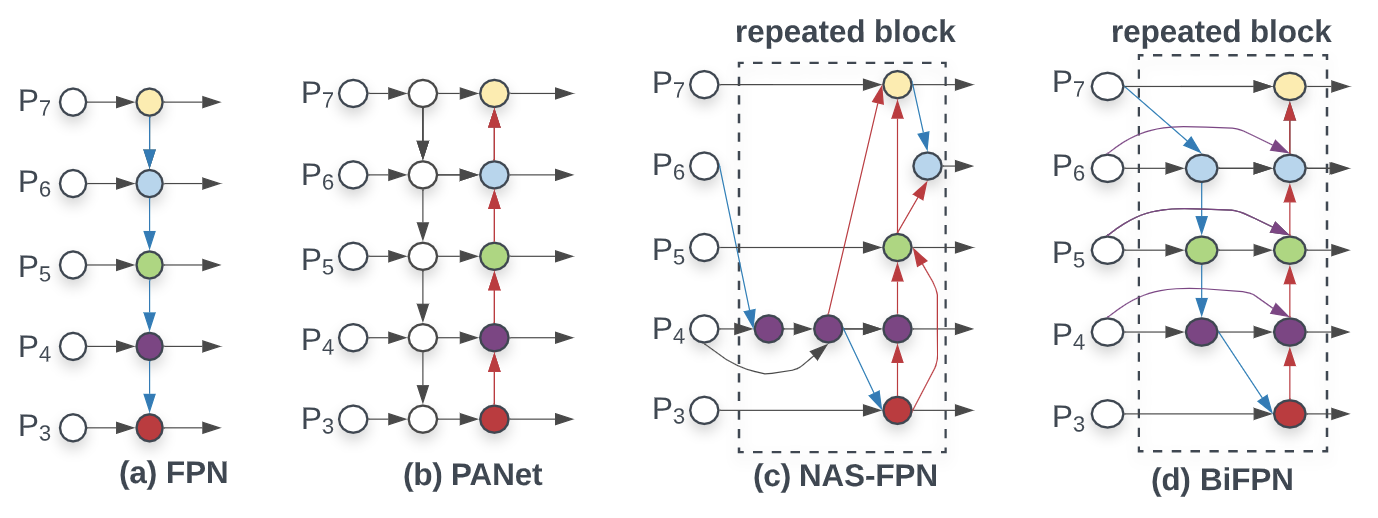
\includegraphics[width=0.8\textwidth]{img/chapters/estado-del-arte/comparativa_fpn+panet+nas-fpn+bifpn.png}
\caption{\label{fig:comparativa-bifpn}Comparativa entre biFPN y las demás redes de características previas}
\end{figure}

Para mejorar aún más la eficiencia, EfficientDet plantea una nueva técnica de fusión rápida normalizada. Las propuestas tradicionales generalmente tratan todas las características de entrada al \gls{fpn} por igual, incluso aquellas con diferentes resoluciones. Sin embargo, se observa que las características de entrada en diferentes resoluciones a menudo tienen contribuciones desiguales a las características de salida. Por lo tanto, agregando un peso adicional para cada característica de entrada se permite que la red aprenda la importancia de cada una. EfficientDet también propone reemplazar todas las circunvoluciones regulares con circunvoluciones separables en profundidad menos costosas. Con estas optimizaciones, Bi\gls{fpn} mejora aún más la precisión en un 4\%, al tiempo que reduce el coste de cálculo en un 50\%.

Una tercera optimización implica lograr mejores compensaciones de precisión y eficiencia bajo diferentes limitaciones de recursos. Escalar conjuntamente la profundidad, el ancho y la resolución de una red puede mejorar significativamente la eficiencia del reconocimiento de imágenes. EfficientDet ofrece un nuevo método de escalado compuesto para detectores de objetos, que escala conjuntamente la resolución/profundidad/ancho. Cada componente de la red, es decir, el backbone, la característica y la red de predicción de cuadro/clase, tendrá un único factor de escala compuesto que controla todas las dimensiones de escala utilizando reglas basadas en heurísticas. Este enfoque permite determinar fácilmente cómo escalar el modelo calculando el factor de escala para las restricciones de recursos de destino dadas.

Combinando el nuevo backbone y Bi\gls{fpn}, surge una línea de base EfficientDet-D0 de tamaño pequeño y aplicando una escala compuesta para obtener EfficientDet-D1 a D7. Cada modelo consecutivo tiene un coste computacional más alto, que cubre una amplia gama de restricciones de recursos desde 3 mil millones de \gls{flops} hasta 300 mil millones de \gls{flops}, proporcionando una mayor precisión.

\subsection{YOLOv4}
\label{subsec:yolov4}

\gls{yolo} es uno de los algoritmos de detección de objetos más eficientes que existen. La primera versión fue publicada por Joseph Redmon \cite{redmon2016look} en 2016 y la implementación más reciente \cite{bochkovskiy2020yolov4} está liderada por Alexey Bochkovsky. Predice tanto la posición (representada como un cuadro delimitador) como la clasificación de objetos en imágenes.

\gls{yolo} tiene como objetivo encontrar las siguientes variables en una imagen:

\begin{itemize}
    \item $(bx, by)$ - el centro de un cuadro delimitador
    \item $(bw, bh)$ - el ancho y alto de un cuadro delimitador
    \item $c$ - la clase del objeto
    \item $P_c$ - la probabilidad de que haya un objeto de clase $c$ en el cuadro
\end{itemize}

\gls{yolo} divide la imagen en una imagen de 19x19, donde cada celda predice 5 cuadros delimitadores de la forma $y = (Pc, bx, by, bw, bh, c)$. Esto da $19x19x5 = 1.805$ cuadros delimitadores diferentes por imagen. La eliminación de las cajas con un $Pc$ bajo se denomina \textit{non-max suppression}.

La principal diferencia entre \gls{yolov4} y las implementaciones anteriores es el enfoque en la velocidad. El objetivo del nuevo algoritmo \gls{yolo} es que cualquier persona que tenga una \gls{gpu} decente pueda aplicar el algoritmo para lograr una precisión increíble para el reconocimiento de imágenes que se ejecuta en tiempo real. En la figura \ref{fig:yolov4-speed-accuracy-vs-others}, se muestran los resultados de la comparación entre \gls{yolov4} y otras arquitecturas, donde es evidente que \gls{yolov4} supera a la mayoría de las otras redes neuronales en términos de precisión promedio y lo hace a más del doble de la velocidad de fotogramas. Esto diferencia mucho a \gls{yolov4} de los otros algoritmos, ya que se puede utilizar en la clasificación de objetos en tiempo real con una precisión casi humana. Por ejemplo, la \gls{cnn} puede diferenciar entre automóviles, bicicletas y camiones que circulan por una carretera. Con su alta velocidad y precisión sorprendentemente buena, \gls{yolo} es ampliamente adoptado y, como tal, es un éxito.

\begin{figure}[ht]
\centering
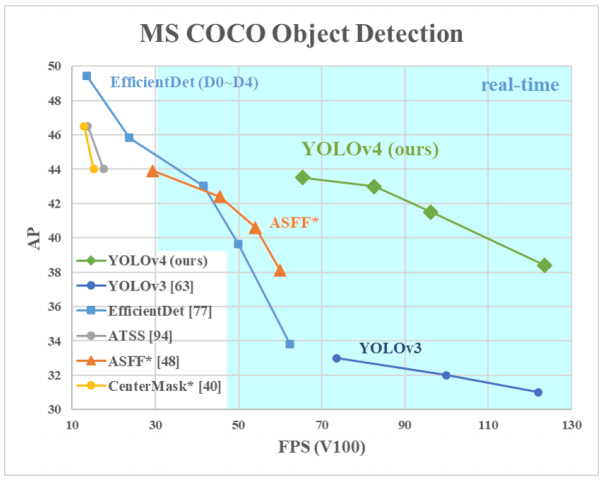
\includegraphics[width=0.45\textwidth]{img/chapters/estado-del-arte/yolov4-vs-others.png}
\caption{\label{fig:yolov4-speed-accuracy-vs-others}Comparativa velocidad y precisión de YOLOv4 frente a otras arquitecturas}
\end{figure}

\subsubsection*{Estructura de un detector de objetos}
\label{subsubsec:estructura-detector-objetos}

Todos los detectores de objetos toman una imagen como entrada y comprimen las características a través de una red neuronal convolucional. En la clasificación de imágenes, estos backbones son el final de la red y se pueden hacer predicciones a partir de ellas. En la detección de objetos, es necesario dibujar varios cuadros delimitadores alrededor de las imágenes junto con la clasificación, por lo que las capas de características convolucional del backbone deben mezclarse unas de otras. La combinación de capas de características del backbone ocurre en el neck.

También es útil dividir los detectores de objetos en dos categorías: detectores de una etapa y detectores de dos etapas. La detección ocurre en el head. Los detectores de dos etapas desacoplan la tarea de localización y clasificación de objetos para cada cuadro delimitador. Los detectores de una etapa hacen las predicciones para la localización y clasificación de objetos al mismo tiempo. \gls{yolo} es un detector de una etapa, por lo tanto, solo mira una vez.

\begin{figure}[ht]
\centering
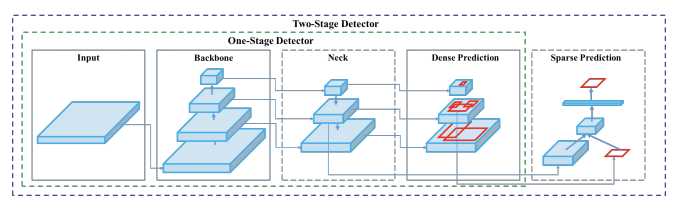
\includegraphics[width=0.9\textwidth]{img/chapters/estado-del-arte/one-two-stage-detector.png}
\caption{\label{fig:one-two-stage-detector}Arquitectura de detectores de objetos de una y dos etapas}
\end{figure}

\subsubsection*{Backbone de YOLOv4}
\label{subsubsec:yolov4-backbone}

El backbone de la red de un detector de objetos típicamente suele estar preentrenada en la clasificación de ImageNet \cite{russakovsky2015imagenet}. El entrenamiento previo significa que los pesos de la red ya se han adaptado para identificar características relevantes en una imagen, aunque se modificarán en la nueva tarea de detección de objetos.

Los autores consideraron los siguientes backbones para el detector de objetos \gls{yolov4}:

\begin{itemize}
    \item CSPResNext50
    \item CSPDarknet53
    \item EfficientNet-B3
\end{itemize}

CSPResNext50 y CSPDarknet53 se basan en DenseNet. DenseNet fue diseñado para conectar capas en redes neuronales convolucionales con las siguientes objetivos: aliviar el problema del gradiente de desaparición (es difícil retropropulsar señales de pérdida a través de una red muy profunda), reforzar la propagación de características, alentar a la red a reutilizar características y reducir el número de parámetros de red.

En CSPResNext50 y CSPDarknet53, DenseNet se ha editado para separar el mapa de características de la capa base copiándolo y enviando una copia a través del bloque denso y enviando otra directamente a la siguiente etapa. La idea con CSPResNext50 y CSPDarknet53 es eliminar los cuellos de botella computacionales en DenseNet y mejorar el aprendizaje al pasar una versión sin editar del mapa de características.

EfficientNet fue diseñado por Google Brain para estudiar principalmente el problema de escala de las redes neuronales convolucionales. Hay muchas decisiones que puede tomar al escalar su ConvNet, incluido el tamaño de entrada, la escala de ancho, la escala de profundidad y la escala de todo lo anterior. El artículo \cite{tan2020efficientdet} postula que hay un punto óptimo para todos estos y, a través de la búsqueda, lo encuentran.

EfficientNet supera a las otras redes de tamaño comparable en clasificación de imágenes. Los autores de \gls{yolov4} postulan, sin embargo, que las otras redes pueden funcionar mejor en la configuración de detección de objetos y deciden experimentar con todas ellas.

En base a los resultados experimentales, la red \gls{yolov4} final implementa CSPDarknet53 para el backbone.

\subsubsection*{Neck de YOLOv4}
\label{subsubsec:yolov4-neck}

El siguiente paso en la detección de objetos es mezclar y combinar las características formadas en el backbone de ConvNet para prepararse para el paso de detección. \gls{yolov4} considera algunas opciones para el cuello que incluyen: \gls{fpn}, \gls{pan}, \gls{nas}-\gls{fpn}, Bi\gls{fpn}, \gls{asff} y \gls{sfam}.



Los componentes del neck normalmente fluyen hacia arriba y hacia abajo entre las capas y conectan solo las pocas capas al final de la red convolucional.

Como se pudo observar en la figura \ref{fig:comparativa-bifpn}, EfficientDet utiliza la búsqueda de arquitectura neuronal para encontrar la mejor forma de bloques en la parte del neck de la red, llegando a \gls{nas}-\gls{fpn}. Los autores de EfficientDet lo modificaron ligeramente para hacer que la arquitectura sea más intuitiva (y probablemente funcione mejor en sus conjuntos de desarrollo).

\gls{yolov4} elige \gls{pan}et para la agregación de funciones de la red. No hay escrito mucho sobre el fundamento de esta decisión, y dado que \gls{nas}-\gls{fpn} y Bi\gls{fpn} se escribieron al mismo tiempo, se prevé que sea un área de investigación futura.

Además, \gls{yolov4} agrega un bloque \gls{spp} después de CSPDarknet53 para aumentar el campo receptivo y separar las características más importantes del backbone.

\subsubsection*{Head de YOLOv4}
\label{subsubsec:yolov4-head}

\gls{yolov4} implementa el mismo head \gls{yolo} que \gls{yolo}v3 \cite{redmon2018yolov3} para la detección con el anchor basado en pasos de detección y tres niveles de granularidad de detección.

\section{Algoritmos de seguimiento de objetos}
\label{sec:tecnicas-utilizadas-tracking}

\subsection{FairMOT}
\label{subsec:fairmot}

\gls{fairmot}

\cite{zhang2020fair}

\newpage

\subsection{SORT}
\label{subsec:sort}

\gls{sort}

\cite{Bewley_2016}

\newpage

\subsection{DeepSORT}
\label{subsec:deepsort}

\gls{deepsort}

\cite{Wojke2017simple}

Explicar que se trata de un algoritmo que combina El filtro de Kalman con el algoritmo húngaro.

\begin{figure}[ht]
\centering
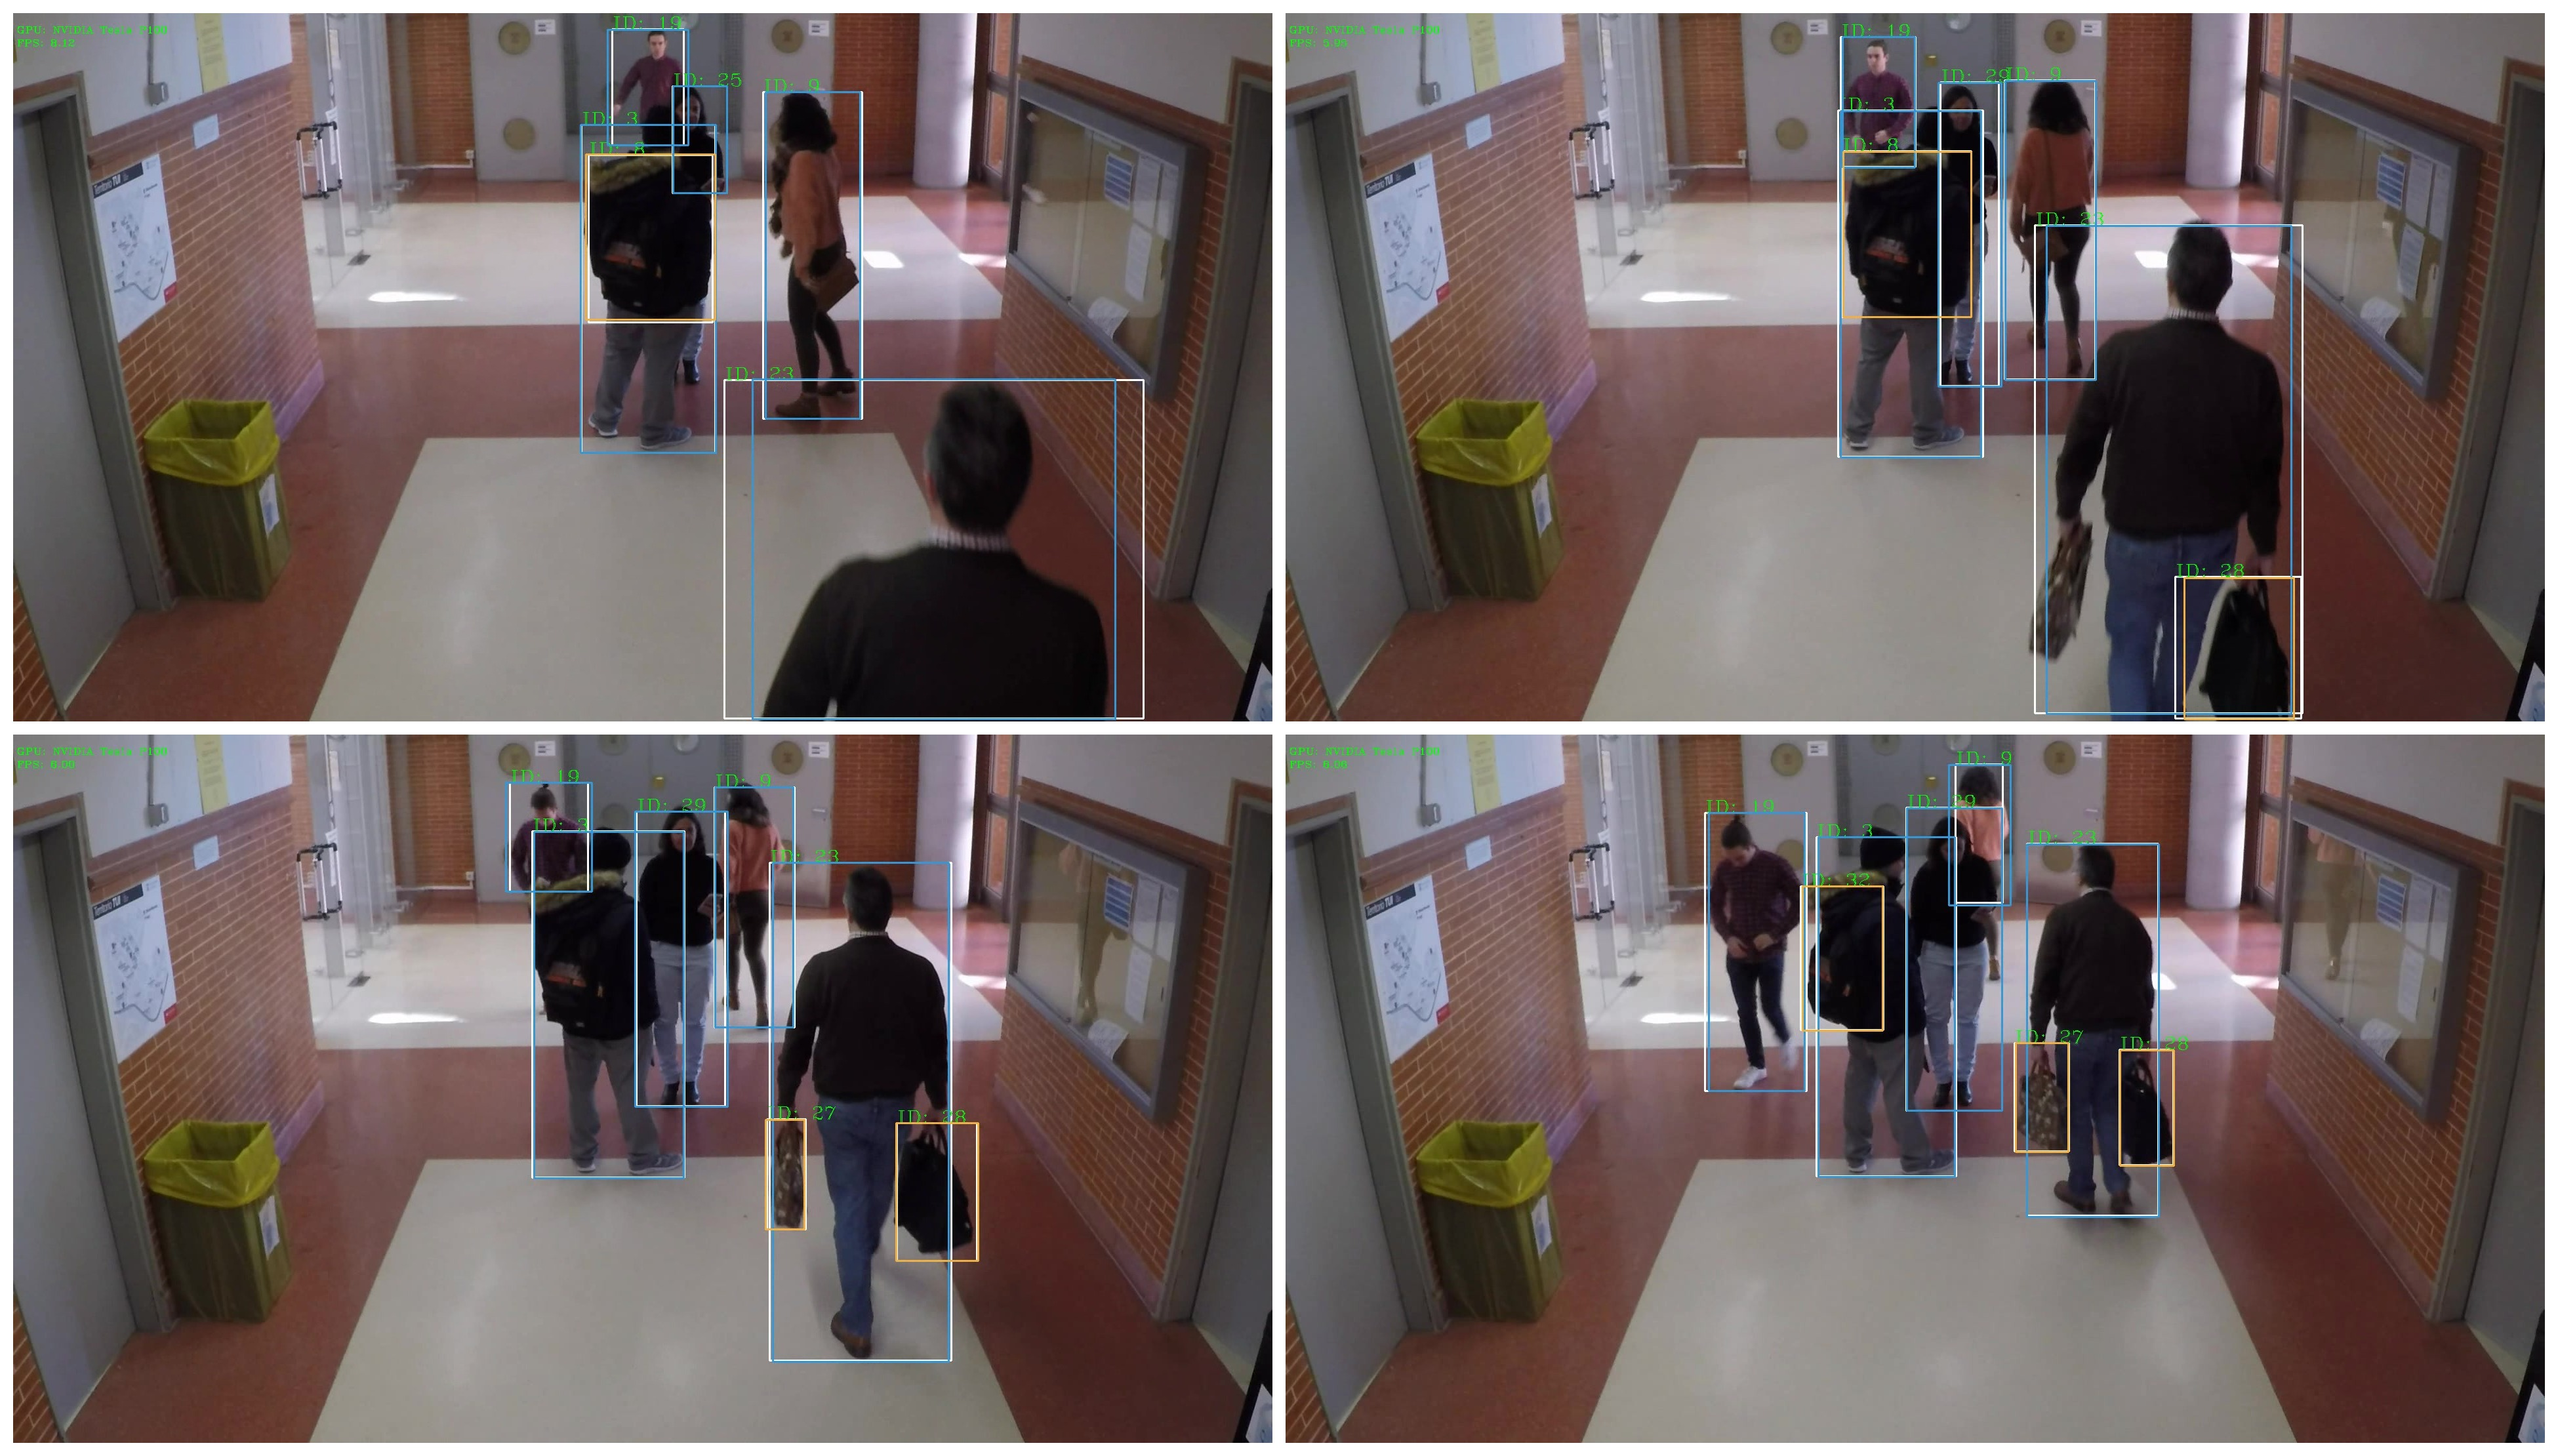
\includegraphics[width=1\textwidth]{img/chapters/algoritmos/deepsort-example.png}
\caption{\label{fig:tracking-example}Funcionamiento de Deepsort}
\end{figure}

En azul y naranja las detecciones, deepsort cuadros delimitadores blancos.

\subsubsection{Filtro de Kalman}
\label{subsubsec:kalman-filter}

Explicar filtro de Kalman

\subsubsection{Algoritmo húngaro}
\label{subsubsec:hungarian-algorithm}

Explicar algoritmo húngaro.

\newpage

\section{Conclusiones}
\label{sec:conclu-sota}

\begin{table}[ht]
\centering
\caption{Velocidad y precisión YOLOv4 y SSD con Maxwell GPU: GTX Titan X (Maxwell) o Tesla M40 GPU, datos extraídos de \cite{bochkovskiy2020yolov4} y \cite{Liu_2016}}
\label{tab:maxwell-speed-accuracy}
\begin{tabular}{llcccc}
\hline
\textbf{Method} & \textbf{Backbone}      & \textbf{Size} & \textbf{FPS}    & \textbf{AP}     & \textbf{AP50}   \\ \hline
YOLOv4          & CSPDarknet-53          & 416           & 38 (M)          & 41,2\%          & 62,8\%          \\
\textbf{YOLOv4} & \textbf{CSPDarknet-53} & \textbf{512}  & \textbf{31 (M)} & \textbf{43,0\%} & \textbf{64,9\%} \\
YOLOv4          & CSPDarknet-53          & 608           & 23 (M)          & 43,5\%          & 65,7\%          \\
                &                        &               &                 &                 &                 \\
SSD             & VGG-16                 & 300           & 43 (M)          & 25,1\%          & 43,1\%          \\
\textbf{SSD}    & \textbf{VGG-16}        & \textbf{512}  & \textbf{22 (M)} & \textbf{28,8\%} & \textbf{48,5\%} \\ \hline
\end{tabular}
\end{table}

\begin{table}[ht]
\centering
\caption{Velocidad y precisión YOLOv4 y Faster R-CNN con Pascal GPU: Titan X (Pascal), Titan Xp, GTX 1080 Ti, o Tesla P100 GPU, datos extraídos de \cite{bochkovskiy2020yolov4} y \cite{ren2016faster}}
\label{tab:pascal-speed-accuracy}
\begin{tabular}{llcccc}
\hline
\textbf{Method}       & \textbf{Backbone}      & \textbf{Size} & \textbf{FPS}     & \textbf{AP}     & \textbf{AP50}   \\ \hline
\textbf{YOLOv4}       & \textbf{CSPDarknet-53} & \textbf{416}  & \textbf{54 (P)}  & \textbf{41,2\%} & \textbf{62,8\%} \\
YOLOv4                & CSPDarknet-53          & 512           & 43 (P)           & 43,0\%          & 64,9\%          \\
YOLOv4                & CSPDarknet-53          & 608           & 33 (P)           & 43,5\%          & 65,7\%          \\
                      &                        &               &                  &                 &                 \\
\textbf{Faster R-CNN} & \textbf{ResNet-50}     & \textbf{—}    & \textbf{9,4 (P)} & \textbf{39,8\%} & \textbf{59,2\%} \\ \hline
\end{tabular}
\end{table}

\begin{table}[ht]
\centering
\caption{Velocidad y precisión YOLOv4 y EfficientDet con Volta GPU: Titan Volta or Tesla V100 GPU, datos extraídos de \cite{bochkovskiy2020yolov4} y \cite{tan2020efficientdet}}
\label{tab:volta-speed-accuracy}
\begin{tabular}{llcccc}
\hline
\textbf{Method}          & \textbf{Backbone}      & \textbf{Size}        & \textbf{FPS}         & \textbf{AP}          & \textbf{AP50}        \\ \hline
YOLOv4                   & CSPDarknet-53          & 416                  & 96 (M)               & 41,2\%               & 62,8\%               \\
\textbf{YOLOv4}          & \textbf{CSPDarknet-53} & \textbf{512}         & \textbf{83 (M)}      & \textbf{43,0\%}      & \textbf{64,9\%}      \\
YOLOv4                   & CSPDarknet-53          & 608                  & 62 (M)               & 43,5\%               & 65,7\%               \\
                         &                        & \multicolumn{1}{l}{} & \multicolumn{1}{l}{} & \multicolumn{1}{l}{} & \multicolumn{1}{l}{} \\
\textbf{EfficientDet-D0} & \textbf{Efficient-B0}  & \textbf{512}         & \textbf{62,5 (M)}    & \textbf{33,8\%}      & \textbf{52,2\%}      \\
EfficientDet-D1          & Efficient-B1           & 640                  & 50,0 (M)             & 39,6\%               & 58,6\%               \\
EfficientDet-D2          & Efficient-B2           & 768                  & 41,7 (M)             & 43,0\%               & 62,3\%               \\
EfficientDet-D3          & Efficient-B3           & 896                  & 23,8 (M)             & 45,8\%               & 65,0\%               \\ \hline
\end{tabular}
\end{table}

\chapter{Desarrollo algoritmo de objetos abandonados}
\label{cha:desarrollo}

\section{Introducción}
\label{sec:intro-alg-abandono}

\section{Desarrollo del algoritmo}
\label{sec:alg-abandono}


\begin{table}[!h]
\centering
\begin{tabular}{|c|c|c|c|c|}
\hline
Esto & es & una & tabla & sencilla \\ \hline
1    & 2  & 3   & 4     & 5        \\ \hline
6    & 7  & 8   & 9     & 10       \\ \hline
11   & 12 & 13  & 14    & 15       \\ \hline
\end{tabular}
\caption{Esto es una tabla ejemplo}
\label{tab:my-table}
\end{table}

\section{Conclusiones}
\label{sec:conclu-alg-abandono}

\chapter{Resultados}
\label{cha:resultados}

Aquí se mostrarán los resultados del proyecto \ldots

Como dijo \cite{einstein} \ldots

\section{Introducción}
\label{sec:intro-resultados}

\section{Entorno experimental}
\label{sec:desarrollo-resultados}

\subsection{Bases de datos utilizadas}
\label{subsec:bases-datos}

\subsection{Métricas de calidad}
\label{subsec:metricas-calidad}

\subsection{Estrategia y metodología de experimentación}
\label{subsec:estrategia-metodologia}

\section{Resultados experimentales}
\label{sec:resultados-experimentales}

\section{Conclusiones}
\label{sec:conclu-resultados}

\chapter{Conclusiones y líneas futuras}
\label{cha:concl-lineas-futuras}

En esta sección se hablará sobre futuros proyectos derivados de éste \ldots

\section{Conclusiones}
\label{sec:conclusiones-finales}

\section{Líneas futuras}
\label{sec:lineas-futuras}

% Biblio
\bibliography{biblio/biblio.bib}
\bibliographystyle{IEEEtran}

% Anexos
\begin{appendices}
\chapter{Pliego de condiciones}
\label{cha:pliego-de-condiciones}

\section{Introducción}

En este apartado se evaluaran las condiciones para poner en marcha el software que se ha especificado en los apartados anteriores. Cabe resaltar el carácter de este proyecto, en el que se ha diseñado una colección de funciones que facilitan al programador la correcta adquisición de datos sonoros, y por lo tanto no aplican las condiciones técnicas o ambientales que pudieran afectarle, ya que las impone los requerimientos las aplicaciones que en un futuro se le quiera dar a este proyecto.

Solamente afectan las condiciones de configuración hardware o software donde se quiera aplicar el programa informático.

\section{Requisitos de hardware}

\subsection{Requisitos mínimos}
\begin{itemize}
  \item Utilización de un PC de 32 bits de escritorio con tarjeta de sonido.
  \item Un mínimo de 384 MB de memoria RAM.
  \item Al menos 100 MB de memoria libre en disco duro.
\end{itemize}

\subsection{Requisitos de hardware recomendados}
Estos requisitos son necesarios para implementar algoritmos de localización basados en onda sonora.
\begin{itemize}
  \item CPU de 64 bits con 4 Cores o más.
  \item Sistema de adquisición con 8 canales o más.
  \item Utilización de al menos 4 Gb de memoria RAM.
\end{itemize}

\section{Condiciones hardware}

El sistema de adquisición que se propone hace uso de 4 hilos independientes en la adquisición en tiempo real. Es por esta razón que se recomienda sistemas multiprocesador, que permitan realizar las tareas de cada hilo de manera independiente.

Se precisa de un sistema de adquisición de audio profesional para la adquisición del audio proveniente de cada micrófono para ejecutar el algoritmo de localización. Además por esta razón y porque se van a generar gran cantidad de datos a procesar en la memoria RAM del equipo, es necesaria la utilización de un volumen importante de memoria RAM, se recomienda que la cifra de partida sean 4 Gb que es la cifra máxima que un sistema operativo de 32 bits basado en Linux puede direccionar.

Se recomienda tener 100 MB de disco duro libre para poder hacer grabaciones de corta duración. Es altamente recomendable disponer de 10 GB libres si se van a realizar grabaciones multicanal y de larga duración.
 
\section{Requisitos de software}

\subsection{Requisitos mínimos}
\begin{itemize}
  \item Utilización de un sistema operativo Ubuntu 12.04.
  \item Librería \texttt{Rtaudio}.
  \item Librería \texttt{SNDFile}.
  \item Para el desarrollo del algoritmo de localización se deben utilizar las librerías propias del grupo GEINTRA.
\end{itemize}

\subsection{Requisitos de software recomendados}
\begin{itemize}
  \item Utilización de un sistema operativo de 64 bits, Ubuntu 12.04 o superior.
\end{itemize}

\section{Condiciones software}

En este apartado software se recomienda utilizar el sistema operativo Ubuntu 12.04 al ser LTS, y proporcionar la compatibilidad con las nuevas librerías Qt para realizar profiling mediante KCachegrind.

En el caso de disponer un sistema hardware con una memoria RAM superior a 4 GB es necesario utilizar, una verisón de Ubuntu de 64 bits para poder direccionarla. Es muy recomendable esta opción para poder adquirir y procesar sonido multicanal.

\newpage
\section{Condiciones generales}

La utilización de esta librería supone la posibilidad de ejecutar cualquier programa de procesamiento sobre ella que tenga en cuenta las siguientes condiciones:

\begin{itemize}
  \item El ancho de banda de las señales acústicas está condicionado por el rango que permita la tarjeta de adquisición a utilizar, por lo general cumple aproximadamente la del espectro del oído humano, de 20 a 20000 Hz.
  \item El número de canales a utilizar lo limita la tarjeta de adquisición, la librería está preparada para adquirir, sea cual sea el rango multicanal.
  \item Ante cualquier uso de esta librería deberá tenerse en cuenta el reconocimiento (BY), que no es comercial (NC), y que las obras derivadas se compartan de igual manera (SA).

\end{itemize}

\chapter{Presupuesto}
\label{cha:presupuesto}

\section{Equipo de trabajo}

Para la realización del proyecto se va a necesitar un Ingeniero de Telecomunicaciones.

\section{Timing}

Las fases necesarias para la realización del desarrollo son las siguientes.

\begin{itemize}
  \item Configuración del hardware (0,5 meses)
  
  \begin{itemize}
    \item Instalación de sistema operativo, librerías, IDE. (0,25 meses)
    \item Configuración y puesta en marcha. (0,25 meses)
  \end{itemize}
  
\item Diseño e implementación de los módulos software necesarios (6 meses):
  
  \begin{itemize}
    
  \item Diseño e implementación de librerías de soporte para la
    reproducción y adquisición de audio multicanal temporizado (tiempos
    fijos) (2 mes).
    
  \item Diseño e implementación de librerías de soporte para la
    adquisición, reproducción y procesamiento de audio multicanal
    continuo (tiempo indefinido) (4 mes).
    
  \end{itemize}
  

\item Evaluación del sistema de procesamiento de audio multicanal (1,5 meses):
  
  \begin{itemize}
    
  \item Adaptación del algoritmo SRP. (0,5 meses)
  
  \item Evaluación del sistema de adquisición sobre la librería de tiempo real (1 mes)
    
    \end{itemize}
  
\item Documentación

\end{itemize}

Por supuesto, las fases de diseño, desarrollo, pruebas y documentación
son cíclicas y abarcan todo el periodo de la vida del proyecto.


\section{Presupuesto total}

Por todo lo anterior, supone una duración de 8 meses naturales con un coste de 12.000 \euro (sin IVA).


\chapter{Manual de usuario e instalación}
\label{cha:manual-usuario}

\section{Introducción}
\label{sec:intro-manual-de-usuario}

Blah, blah, blah\ldots


\section{Manual}
\label{sec:sec-manual-de-usuario}

Pues eso.


\section{Ejemplos de inclusión de fragmentos de código fuente}
\label{sec:codigo-fuente}

Ahora compila usando \texttt{gcc}:

\begin{enumerate}
\item bla bla:

\begin{lstlisting}
$ python object_tracker.py --video ./data/video/video1.avi

\end{lstlisting}

\end{enumerate}



\end{appendices}

% Contraportada

\includepdf[pages={6}]{cover/portada.pdf}

\end{document}
